\chapter{Linear Multistep Methods}


\begin{intro}
  In the previous methods we obtained the value after the next time
  step always by using \emph{one} initial value at the beginning of
  the current time interval, possibly with the
  help of intermediate steps. These methods often are accused to have
  a higher computation time than methods which use several previous
  points, the argument being that function values at these points have
  been computed already. Such methods using values of several time steps in
  the past are called multistep methods. They are constructed such
  that using more steps yields a method of higher order.

  We will begin this chapter by introducing some of the
  formulas. Afterwards, we will study their stability and convergence
  properties.
\end{intro}

\begin{example}[Adams-Moulton formulas]
  \label{ex:lmm:2}  
  \index{Adams-Moulton methods} Basically, there are two construction
  principles for the multistep methods: Quadrature and numerical
  differentiation.  We postpone the latter to example~\ref{ex:lmm:3}
  and deal with the former for now.  As first example we choose the
  class of Adams-Moulton methods for which the integral from point
  $t_{k-1}$ to point $t_{k}$ is approximated by a quadrature of the
  points $t_{k-\lmms}$ to $t_k$, hence
  \begin{gather}
    \label{eq:lmm:16}
    y_k = y_{k-1} + \sum_{r=0}^\lmms f_{k-r} \int_{t_{k-1}}^{t_k}
    L_r(t) \dt,
  \end{gather}
  where $f_j$ denotes the function value $f(t_j, y_j)$ and $L_r(t)$
  the Lagrange interpolation polynomial to point $t_r$ with respect to
  the points $t_{k-\lmms},\dots,t_k$.  This is shown in
  Figure~\ref{fig:lmm:adams-moulton}.
  \begin{figure}[tbp]
    \begin{center}
      \includegraphics[width=.9\textwidth]{fig/adams-moulton.tikz}
    \end{center}
    \caption{The quadrature of Adams-Moulton formulas: the
      integration interval is marked by the wavy line in the end. The support 
			points of the quadrature are stated under the line.}
    \label{fig:lmm:adams-moulton}
  \end{figure}
  Since the integral involves the point being computed itself, these
  methods are implicit. The first of these are
  \begin{align*}
  y_k &= y_{k-1} + h f_k \\
  y_k &= y_{k-1} + \frac12h
        \bigl( f_k + f_{k-1}\bigr)\\
  y_k &= y_{k-1} +
        \frac1{12}h \bigl( 5f_k + 8 f_{k-1} -  f_{k-2}\bigr)\\
  y_k &= y_{k-1} +
        \frac1{24}h \bigl(9f_k+19 f_{k-1}-5 f_{k-2}+ f_{k-3}\bigr)
\end{align*}

%%% Local Variables:
%%% mode: latex
%%% TeX-master: "../notes"
%%% End:
  
\end{example}

\begin{example}[Adams-Bashforth formulas]
  \label{ex:lmm:1}
  \index{Adams-Bashforth methods} With the same principle we obtain
  explicit methods by omitting the point in time $t_k$ in the
  definition of the interpolation polynomial. See
  Figure~\ref{fig:lmm:adams-bashforth}.
  \begin{figure}[tbp]
    \begin{center}
      \includegraphics[width=.9\textwidth]{fig/adams-bashforth.tikz}
    \end{center}
    \caption{The quadrature of Adams-Bashforth formulas: the
      integration interval is marked by the wavy line in the end. The support 
			points of the quadrature are stated under the line.}
    \label{fig:lmm:adams-bashforth}
  \end{figure}
  This yields quadrature formulas of the form
  \begin{gather}
    \label{eq:lmm:17}
    y_k = y_{k-1} + \sum_{r=1}^\lmms f_{k-r} \int_{t_{k-1}}^{t_k}
    L_r(t) \dt.
  \end{gather}
  Again, we list the first few:
  \begin{tikzpicture}
  \draw[snake=snake](7,0) -- (8,0);
  \draw(5,0) -- (7,0);
  % \draw(2,0) -- (3,0);
  \draw[dotted](0,0)--(3,0);
  \draw[dashed](3,0)--(5,0);
  
  \draw(8,-.1) --(8,.1) node[anchor=south]{$t_{k}$};
  \draw(7,-.1) node[anchor=north]{$t_{k-1}$} --(7,.1);
  \draw(6,-.1) node[anchor=north]{$t_{k-2}$} --(6,.1);
  \draw(5,-.1) node[anchor=north]{$t_{k-3}$} --(5,.1);
  
  \draw(3,-.1) node[anchor=north]{$t_{k-\lmms}$} --(3,.1);
  % \draw(2,-.1) --(2,.1) node[anchor=south]{$t_{k-\lmms-1}$};
\end{tikzpicture}

\end{example}

\begin{example}
  \label{ex:lmm:3}
  \index{BDF methods} Backward differencing formulas (BDF) are as well
  based on Lagrange interpolation at the points $t_{k-\lmms}$ to
  $t_k$. In contrast to Adams formulas they do not use quadrature for
  the right hand side, but rather the derivative of the interpolation
  polynomial in the point $t_k$.  Using Lagrange interpolation
  polynomials $L_i(t)$, we let
  \begin{gather*}
    y(t) = \sum_{r=0}^\lmms y_{n-r} L_{n-r}(t),
  \end{gather*}
  where $y_n$ is still to determine. Now we assume that $y$ solves the ODE
  in point $t_n$, hence
  \begin{gather*}
    y'(t_n) = f(t_n, y_n) = \sum_{r=0}^\lmms y_{n-r} L'_{n-r}(t_n).
  \end{gather*}
  This yields the following schemes:
  \begin{align*}
  y_k-y_{k-1} &= h f_k \\
  y_k-\tfrac43 y_{k-1} + \tfrac13y_{k-2} &= \tfrac23 h f_k \\
  y_k-\tfrac{18}{11} y_{k-1} + \tfrac{9}{11} y_{k-2} -
  \tfrac{2}{11} y_{k-3}
              &= \tfrac6{11} h f_k \\
  y_k-\tfrac{48}{25} y_{k-1} + \tfrac{36}{25} y_{k-2} -
  \tfrac{16}{25} y_{k-3} + \tfrac{3}{25} y_{k-4}
              &= \tfrac{12}{25} h f_k
\end{align*}

%%% Local Variables:
%%% mode: latex
%%% TeX-master: "../notes"
%%% End:

\end{example}

\begin{remark}
  We know from introduction to numerical analysis, that the numerical
  differentiation and the extrapolation, the evaluation of
  interpolation polynomials outside of the interval which is spanned
  through the interpolation points, are not stable.  Therefore, we
  expect stability problems for the Adams-Bashforth and BDF
  methods. Moreover we remember that Lagrange interpolation with
  equidistant support points is unstable for a high
  polynomials. Therefore, we also expect that all methods above
  perform well only with moderate order.
\end{remark}

%%%%%%%%%%%%%%%%%%%%%%%%%%%%%%%%%%%%%%%%%%%%%%%%%%%%%%%%%%%%%%%%%%%%%%
%%%%%%%%%%%%%%%%%%%%%%%%%%%%%%%%%%%%%%%%%%%%%%%%%%%%%%%%%%%%%%%%%%%%%%
\section{Definition and consistency of LMM}
%%%%%%%%%%%%%%%%%%%%%%%%%%%%%%%%%%%%%%%%%%%%%%%%%%%%%%%%%%%%%%%%%%%%%%
%%%%%%%%%%%%%%%%%%%%%%%%%%%%%%%%%%%%%%%%%%%%%%%%%%%%%%%%%%%%%%%%%%%%%%

\chapter{Linear Multistep Methods}


\begin{intro}
  In the previous methods we obtained the value after the next time
  step always by using \emph{one} initial value at the beginning of
  the current time interval, possibly with the
  help of intermediate steps. These methods often are accused to have
  a higher computation time than methods which use several previous
  points, the argument being that function values at these points have
  been computed already. Such methods using values of several time steps in
  the past are called multistep methods. They are constructed such
  that using more steps yields a method of higher order.

  We will begin this chapter by introducing some of the
  formulas. Afterwards, we will study their stability and convergence
  properties.
\end{intro}

\begin{example}[Adams-Moulton formulas]
  \label{ex:lmm:2}  
  \index{Adams-Moulton methods} Basically, there are two construction
  principles for the multistep methods: Quadrature and numerical
  differentiation.  We postpone the latter to example~\ref{ex:lmm:3}
  and deal with the former for now.  As first example we choose the
  class of Adams-Moulton methods for which the integral from point
  $t_{k-1}$ to point $t_{k}$ is approximated by a quadrature of the
  points $t_{k-\lmms}$ to $t_k$, hence
  \begin{gather}
    \label{eq:lmm:16}
    y_k = y_{k-1} + \sum_{r=0}^\lmms f_{k-r} \int_{t_{k-1}}^{t_k}
    L_r(t) \dt,
  \end{gather}
  where $f_j$ denotes the function value $f(t_j, y_j)$ and $L_r(t)$
  the Lagrange interpolation polynomial to point $t_r$ with respect to
  the points $t_{k-\lmms},\dots,t_k$.  This is shown in
  Figure~\ref{fig:lmm:adams-moulton}.
  \begin{figure}[tbp]
    \begin{center}
      \includegraphics[width=.9\textwidth]{fig/adams-moulton.tikz}
    \end{center}
    \caption{The quadrature of Adams-Moulton formulas: the
      integration interval is marked by the wavy line in the end. The support 
			points of the quadrature are stated under the line.}
    \label{fig:lmm:adams-moulton}
  \end{figure}
  Since the integral involves the point being computed itself, these
  methods are implicit. The first of these are
  \begin{align*}
  y_k &= y_{k-1} + h f_k \\
  y_k &= y_{k-1} + \frac12h
        \bigl( f_k + f_{k-1}\bigr)\\
  y_k &= y_{k-1} +
        \frac1{12}h \bigl( 5f_k + 8 f_{k-1} -  f_{k-2}\bigr)\\
  y_k &= y_{k-1} +
        \frac1{24}h \bigl(9f_k+19 f_{k-1}-5 f_{k-2}+ f_{k-3}\bigr)
\end{align*}

%%% Local Variables:
%%% mode: latex
%%% TeX-master: "../notes"
%%% End:
  
\end{example}

\begin{example}[Adams-Bashforth formulas]
  \label{ex:lmm:1}
  \index{Adams-Bashforth methods} With the same principle we obtain
  explicit methods by omitting the point in time $t_k$ in the
  definition of the interpolation polynomial. See
  Figure~\ref{fig:lmm:adams-bashforth}.
  \begin{figure}[tbp]
    \begin{center}
      \includegraphics[width=.9\textwidth]{fig/adams-bashforth.tikz}
    \end{center}
    \caption{The quadrature of Adams-Bashforth formulas: the
      integration interval is marked by the wavy line in the end. The support 
			points of the quadrature are stated under the line.}
    \label{fig:lmm:adams-bashforth}
  \end{figure}
  This yields quadrature formulas of the form
  \begin{gather}
    \label{eq:lmm:17}
    y_k = y_{k-1} + \sum_{r=1}^\lmms f_{k-r} \int_{t_{k-1}}^{t_k}
    L_r(t) \dt.
  \end{gather}
  Again, we list the first few:
  \begin{tikzpicture}
  \draw[snake=snake](7,0) -- (8,0);
  \draw(5,0) -- (7,0);
  % \draw(2,0) -- (3,0);
  \draw[dotted](0,0)--(3,0);
  \draw[dashed](3,0)--(5,0);
  
  \draw(8,-.1) --(8,.1) node[anchor=south]{$t_{k}$};
  \draw(7,-.1) node[anchor=north]{$t_{k-1}$} --(7,.1);
  \draw(6,-.1) node[anchor=north]{$t_{k-2}$} --(6,.1);
  \draw(5,-.1) node[anchor=north]{$t_{k-3}$} --(5,.1);
  
  \draw(3,-.1) node[anchor=north]{$t_{k-\lmms}$} --(3,.1);
  % \draw(2,-.1) --(2,.1) node[anchor=south]{$t_{k-\lmms-1}$};
\end{tikzpicture}

\end{example}

\begin{example}
  \label{ex:lmm:3}
  \index{BDF methods} Backward differencing formulas (BDF) are as well
  based on Lagrange interpolation at the points $t_{k-\lmms}$ to
  $t_k$. In contrast to Adams formulas they do not use quadrature for
  the right hand side, but rather the derivative of the interpolation
  polynomial in the point $t_k$.  Using Lagrange interpolation
  polynomials $L_i(t)$, we let
  \begin{gather*}
    y(t) = \sum_{r=0}^\lmms y_{n-r} L_{n-r}(t),
  \end{gather*}
  where $y_n$ is still to determine. Now we assume that $y$ solves the ODE
  in point $t_n$, hence
  \begin{gather*}
    y'(t_n) = f(t_n, y_n) = \sum_{r=0}^\lmms y_{n-r} L'_{n-r}(t_n).
  \end{gather*}
  This yields the following schemes:
  \begin{align*}
  y_k-y_{k-1} &= h f_k \\
  y_k-\tfrac43 y_{k-1} + \tfrac13y_{k-2} &= \tfrac23 h f_k \\
  y_k-\tfrac{18}{11} y_{k-1} + \tfrac{9}{11} y_{k-2} -
  \tfrac{2}{11} y_{k-3}
              &= \tfrac6{11} h f_k \\
  y_k-\tfrac{48}{25} y_{k-1} + \tfrac{36}{25} y_{k-2} -
  \tfrac{16}{25} y_{k-3} + \tfrac{3}{25} y_{k-4}
              &= \tfrac{12}{25} h f_k
\end{align*}

%%% Local Variables:
%%% mode: latex
%%% TeX-master: "../notes"
%%% End:

  For an example on how to derive these schemes see the appendix.
\end{example}

\begin{remark}
  We know from introduction to numerical analysis, that the numerical
  differentiation and the extrapolation, the evaluation of
  interpolation polynomials outside of the interval which is spanned
  through the interpolation points, are not stable.  Therefore, we
  expect stability problems for the Adams-Bashforth and BDF
  methods. Moreover, we remember that Lagrange interpolation with
  equidistant support points is unstable for a high-degree
  polynomials. Therefore, we also expect that all methods above
  perform well only with moderate order.
\end{remark}

%%%%%%%%%%%%%%%%%%%%%%%%%%%%%%%%%%%%%%%%%%%%%%%%%%%%%%%%%%%%%%%%%%%%%%
%%%%%%%%%%%%%%%%%%%%%%%%%%%%%%%%%%%%%%%%%%%%%%%%%%%%%%%%%%%%%%%%%%%%%%
\section{Definition and consistency of LMM}
%%%%%%%%%%%%%%%%%%%%%%%%%%%%%%%%%%%%%%%%%%%%%%%%%%%%%%%%%%%%%%%%%%%%%%
%%%%%%%%%%%%%%%%%%%%%%%%%%%%%%%%%%%%%%%%%%%%%%%%%%%%%%%%%%%%%%%%%%%%%%

\chapter{Linear Multistep Methods}


\begin{intro}
  In the previous methods we obtained the value after the next time
  step always by using \emph{one} initial value at the beginning of
  the current time interval, possibly with the
  help of intermediate steps. These methods often are accused to have
  a higher computation time than methods which use several previous
  points, the argument being that function values at these points have
  been computed already. Such methods using values of several time steps in
  the past are called multistep methods. They are constructed such
  that using more steps yields a method of higher order.

  We will begin this chapter by introducing some of the
  formulas. Afterwards, we will study their stability and convergence
  properties.
\end{intro}

\begin{example}[Adams-Moulton formulas]
  \label{ex:lmm:2}  
  \index{Adams-Moulton methods} Basically, there are two construction
  principles for the multistep methods: Quadrature and numerical
  differentiation.  We postpone the latter to example~\ref{ex:lmm:3}
  and deal with the former for now.  As first example we choose the
  class of Adams-Moulton methods for which the integral from point
  $t_{k-1}$ to point $t_{k}$ is approximated by a quadrature of the
  points $t_{k-\lmms}$ to $t_k$, hence
  \begin{gather}
    \label{eq:lmm:16}
    y_k = y_{k-1} + \sum_{r=0}^\lmms f_{k-r} \int_{t_{k-1}}^{t_k}
    L_r(t) \dt,
  \end{gather}
  where $f_j$ denotes the function value $f(t_j, y_j)$ and $L_r(t)$
  the Lagrange interpolation polynomial to point $t_r$ with respect to
  the points $t_{k-\lmms},\dots,t_k$.  This is shown in
  Figure~\ref{fig:lmm:adams-moulton}.
  \begin{figure}[tbp]
    \begin{center}
      \includegraphics[width=.9\textwidth]{fig/adams-moulton.tikz}
    \end{center}
    \caption{The quadrature of Adams-Moulton formulas: the
      integration interval is marked by the wavy line in the end. The support 
			points of the quadrature are stated under the line.}
    \label{fig:lmm:adams-moulton}
  \end{figure}
  Since the integral involves the point being computed itself, these
  methods are implicit. The first of these are
  \begin{align*}
  y_k &= y_{k-1} + h f_k \\
  y_k &= y_{k-1} + \frac12h
        \bigl( f_k + f_{k-1}\bigr)\\
  y_k &= y_{k-1} +
        \frac1{12}h \bigl( 5f_k + 8 f_{k-1} -  f_{k-2}\bigr)\\
  y_k &= y_{k-1} +
        \frac1{24}h \bigl(9f_k+19 f_{k-1}-5 f_{k-2}+ f_{k-3}\bigr)
\end{align*}

%%% Local Variables:
%%% mode: latex
%%% TeX-master: "../notes"
%%% End:
  
\end{example}

\begin{example}[Adams-Bashforth formulas]
  \label{ex:lmm:1}
  \index{Adams-Bashforth methods} With the same principle we obtain
  explicit methods by omitting the point in time $t_k$ in the
  definition of the interpolation polynomial. See
  Figure~\ref{fig:lmm:adams-bashforth}.
  \begin{figure}[tbp]
    \begin{center}
      \includegraphics[width=.9\textwidth]{fig/adams-bashforth.tikz}
    \end{center}
    \caption{The quadrature of Adams-Bashforth formulas: the
      integration interval is marked by the wavy line in the end. The support 
			points of the quadrature are stated under the line.}
    \label{fig:lmm:adams-bashforth}
  \end{figure}
  This yields quadrature formulas of the form
  \begin{gather}
    \label{eq:lmm:17}
    y_k = y_{k-1} + \sum_{r=1}^\lmms f_{k-r} \int_{t_{k-1}}^{t_k}
    L_r(t) \dt.
  \end{gather}
  Again, we list the first few:
  \begin{tikzpicture}
  \draw[snake=snake](7,0) -- (8,0);
  \draw(5,0) -- (7,0);
  % \draw(2,0) -- (3,0);
  \draw[dotted](0,0)--(3,0);
  \draw[dashed](3,0)--(5,0);
  
  \draw(8,-.1) --(8,.1) node[anchor=south]{$t_{k}$};
  \draw(7,-.1) node[anchor=north]{$t_{k-1}$} --(7,.1);
  \draw(6,-.1) node[anchor=north]{$t_{k-2}$} --(6,.1);
  \draw(5,-.1) node[anchor=north]{$t_{k-3}$} --(5,.1);
  
  \draw(3,-.1) node[anchor=north]{$t_{k-\lmms}$} --(3,.1);
  % \draw(2,-.1) --(2,.1) node[anchor=south]{$t_{k-\lmms-1}$};
\end{tikzpicture}

\end{example}

\begin{example}
  \label{ex:lmm:3}
  \index{BDF methods} Backward differencing formulas (BDF) are as well
  based on Lagrange interpolation at the points $t_{k-\lmms}$ to
  $t_k$. In contrast to Adams formulas they do not use quadrature for
  the right hand side, but rather the derivative of the interpolation
  polynomial in the point $t_k$.  Using Lagrange interpolation
  polynomials $L_i(t)$, we let
  \begin{gather*}
    y(t) = \sum_{r=0}^\lmms y_{n-r} L_{n-r}(t),
  \end{gather*}
  where $y_n$ is still to determine. Now we assume that $y$ solves the ODE
  in point $t_n$, hence
  \begin{gather*}
    y'(t_n) = f(t_n, y_n) = \sum_{r=0}^\lmms y_{n-r} L'_{n-r}(t_n).
  \end{gather*}
  This yields the following schemes:
  \begin{align*}
  y_k-y_{k-1} &= h f_k \\
  y_k-\tfrac43 y_{k-1} + \tfrac13y_{k-2} &= \tfrac23 h f_k \\
  y_k-\tfrac{18}{11} y_{k-1} + \tfrac{9}{11} y_{k-2} -
  \tfrac{2}{11} y_{k-3}
              &= \tfrac6{11} h f_k \\
  y_k-\tfrac{48}{25} y_{k-1} + \tfrac{36}{25} y_{k-2} -
  \tfrac{16}{25} y_{k-3} + \tfrac{3}{25} y_{k-4}
              &= \tfrac{12}{25} h f_k
\end{align*}

%%% Local Variables:
%%% mode: latex
%%% TeX-master: "../notes"
%%% End:

  For an example on how to derive these schemes see the appendix.
\end{example}

\begin{remark}
  We know from introduction to numerical analysis, that the numerical
  differentiation and the extrapolation, the evaluation of
  interpolation polynomials outside of the interval which is spanned
  through the interpolation points, are not stable.  Therefore, we
  expect stability problems for the Adams-Bashforth and BDF
  methods. Moreover, we remember that Lagrange interpolation with
  equidistant support points is unstable for a high-degree
  polynomials. Therefore, we also expect that all methods above
  perform well only with moderate order.
\end{remark}

%%%%%%%%%%%%%%%%%%%%%%%%%%%%%%%%%%%%%%%%%%%%%%%%%%%%%%%%%%%%%%%%%%%%%%
%%%%%%%%%%%%%%%%%%%%%%%%%%%%%%%%%%%%%%%%%%%%%%%%%%%%%%%%%%%%%%%%%%%%%%
\section{Definition and consistency of LMM}
%%%%%%%%%%%%%%%%%%%%%%%%%%%%%%%%%%%%%%%%%%%%%%%%%%%%%%%%%%%%%%%%%%%%%%
%%%%%%%%%%%%%%%%%%%%%%%%%%%%%%%%%%%%%%%%%%%%%%%%%%%%%%%%%%%%%%%%%%%%%%

\chapter{Linear Multistep Methods}


\begin{intro}
  In the previous methods we obtained the value after the next time
  step always by using \emph{one} initial value at the beginning of
  the current time interval, possibly with the
  help of intermediate steps. These methods often are accused to have
  a higher computation time than methods which use several previous
  points, the argument being that function values at these points have
  been computed already. Such methods using values of several time steps in
  the past are called multistep methods. They are constructed such
  that using more steps yields a method of higher order.

  We will begin this chapter by introducing some of the
  formulas. Afterwards, we will study their stability and convergence
  properties.
\end{intro}

\begin{example}[Adams-Moulton formulas]
  \label{ex:lmm:2}  
  \index{Adams-Moulton methods} Basically, there are two construction
  principles for the multistep methods: Quadrature and numerical
  differentiation.  We postpone the latter to example~\ref{ex:lmm:3}
  and deal with the former for now.  As first example we choose the
  class of Adams-Moulton methods for which the integral from point
  $t_{k-1}$ to point $t_{k}$ is approximated by a quadrature of the
  points $t_{k-\lmms}$ to $t_k$, hence
  \begin{gather}
    \label{eq:lmm:16}
    y_k = y_{k-1} + \sum_{r=0}^\lmms f_{k-r} \int_{t_{k-1}}^{t_k}
    L_r(t) \dt,
  \end{gather}
  where $f_j$ denotes the function value $f(t_j, y_j)$ and $L_r(t)$
  the Lagrange interpolation polynomial to point $t_r$ with respect to
  the points $t_{k-\lmms},\dots,t_k$.  This is shown in
  Figure~\ref{fig:lmm:adams-moulton}.
  \begin{figure}[tbp]
    \begin{center}
      \includegraphics[width=.9\textwidth]{fig/adams-moulton.tikz}
    \end{center}
    \caption{The quadrature of Adams-Moulton formulas: the
      integration interval is marked by the wavy line in the end. The support 
			points of the quadrature are stated under the line.}
    \label{fig:lmm:adams-moulton}
  \end{figure}
  Since the integral involves the point being computed itself, these
  methods are implicit. The first of these are
  \input{definitions/adams-moulton}  
\end{example}

\begin{example}[Adams-Bashforth formulas]
  \label{ex:lmm:1}
  \index{Adams-Bashforth methods} With the same principle we obtain
  explicit methods by omitting the point in time $t_k$ in the
  definition of the interpolation polynomial. See
  Figure~\ref{fig:lmm:adams-bashforth}.
  \begin{figure}[tbp]
    \begin{center}
      \includegraphics[width=.9\textwidth]{fig/adams-bashforth.tikz}
    \end{center}
    \caption{The quadrature of Adams-Bashforth formulas: the
      integration interval is marked by the wavy line in the end. The support 
			points of the quadrature are stated under the line.}
    \label{fig:lmm:adams-bashforth}
  \end{figure}
  This yields quadrature formulas of the form
  \begin{gather}
    \label{eq:lmm:17}
    y_k = y_{k-1} + \sum_{r=1}^\lmms f_{k-r} \int_{t_{k-1}}^{t_k}
    L_r(t) \dt.
  \end{gather}
  Again, we list the first few:
  \input{definitions/adams-bashforth}
\end{example}

\begin{example}
  \label{ex:lmm:3}
  \index{BDF methods} Backward differencing formulas (BDF) are as well
  based on Lagrange interpolation at the points $t_{k-\lmms}$ to
  $t_k$. In contrast to Adams formulas they do not use quadrature for
  the right hand side, but rather the derivative of the interpolation
  polynomial in the point $t_k$.  Using Lagrange interpolation
  polynomials $L_i(t)$, we let
  \begin{gather*}
    y(t) = \sum_{r=0}^\lmms y_{n-r} L_{n-r}(t),
  \end{gather*}
  where $y_n$ is still to determine. Now we assume that $y$ solves the ODE
  in point $t_n$, hence
  \begin{gather*}
    y'(t_n) = f(t_n, y_n) = \sum_{r=0}^\lmms y_{n-r} L'_{n-r}(t_n).
  \end{gather*}
  This yields the following schemes:
  \input{definitions/bdf}
  For an example on how to derive these schemes see the appendix.
\end{example}

\begin{remark}
  We know from introduction to numerical analysis, that the numerical
  differentiation and the extrapolation, the evaluation of
  interpolation polynomials outside of the interval which is spanned
  through the interpolation points, are not stable.  Therefore, we
  expect stability problems for the Adams-Bashforth and BDF
  methods. Moreover, we remember that Lagrange interpolation with
  equidistant support points is unstable for a high-degree
  polynomials. Therefore, we also expect that all methods above
  perform well only with moderate order.
\end{remark}

%%%%%%%%%%%%%%%%%%%%%%%%%%%%%%%%%%%%%%%%%%%%%%%%%%%%%%%%%%%%%%%%%%%%%%
%%%%%%%%%%%%%%%%%%%%%%%%%%%%%%%%%%%%%%%%%%%%%%%%%%%%%%%%%%%%%%%%%%%%%%
\section{Definition and consistency of LMM}
%%%%%%%%%%%%%%%%%%%%%%%%%%%%%%%%%%%%%%%%%%%%%%%%%%%%%%%%%%%%%%%%%%%%%%
%%%%%%%%%%%%%%%%%%%%%%%%%%%%%%%%%%%%%%%%%%%%%%%%%%%%%%%%%%%%%%%%%%%%%%

\input{definitions/lmm}

\begin{remark}
  \index{step size!constant} The LMM was defined for constant step size
  $h$.  In principle it is possible to implement the method with a
  variable step size but we restrict ourselves to the constant case.
  Notes to the step size control can be found later on in this chapter.
\end{remark}

\begin{remark}
  One-step methods were always denoted by describing how to compute
  $y_1$ from $y_0$. Here, the notation becomes more complicated, but
  sometimes we consider only $y_s$ computed from $y_0,\dots,y_{s-1}$
  implying the same rules for $y_k$ computed from
  $y_{k-\lmms},\dots,y_{k-1}$.
\end{remark}
\input{definitions/lmm-errors}

\begin{lemma}
  Consider the differential equation
  \begin{gather*}
    y' = f(t,y) \qquad y(t_0) = y_0
  \end{gather*}
  where f is given continuously differentiable and $y(t)$ is the exact solution.
  For the local error we obtain

  \begin{gather}
    y(t_k)-y_k = \left( \alpha_0 \identity - h\beta_0 \frac{\partial f}{\partial y}(t_k,\eta) \right)^{-1} (L_h u)(t_k).
  \end{gather}

  Here $\eta$ is a value between $y(t_k)$ and $y_k$ if $f$ is a scalar
	function.
  If $f$ is multidimensional, the matrix 
	$\frac{\partial f}{\partial y}(t_k,\eta)$ is the Jacobi matrix, 
	which rows are evaluated at possible places between
	$y(t_k)$ and $y_k$.
\end{lemma}

\begin{proof}
  Considering the local error we can assume exact initial values 
  and therefore we can transform ~\ref{eq:lmm:4} to:
  \begin{gather*}
    \alpha_\lmms y_k + \sum\limits_{r=1}^\lmms \alpha_{\lmms-r} y(t_{k-r})
    = h \left( \beta_\lmms f_k + \sum\limits_{r=1}^\lmms \beta_{\lmms-r} f_{k-r} \right)
  \end{gather*}
  We transform further:
  \begin{multline*}
    \sum\limits_{r=0}^{\lmms} \left( \alpha_r y(t_{k-r})
      - h \beta_r f(t_{k-r},y(t_{k-r})) \right)
    \\
    - \alpha_0 y(t_k) + h \beta_0 f(t_k, y(t_k)) + \alpha_0 y_k
    - h \beta_0 f(t_k,y_k) = 0.
  \end{multline*}
	We now insert ~\ref{eq:lmm:9} which results in
  \begin{gather*}
    (L_h y)(t_k) = \alpha_0 \left( y(t_k) - y_k \right) - h \beta_0 \left( f(t_k,y(t_k)) - f(t_k,y_k) \right)
    \\
    \left( y(t_k) - y_k \right) \left( \alpha_0 \identity - h \beta_0 \frac{f(t_k,y(t_k)) - f(t_k,y_k)}{y(t_k) - y_k} \right)
  \end{gather*}
  By application of the mean value theorem and 
  subsequent transformation we obtain the statement of the theorem.
\end{proof}

      % \cite[Lemma 2.2, p. 369]{HairerNorsettWanner93}

\input{definitions/lmm-consistency}
\input{theorems/lmm-bramble-hilbert}

\begin{proof}
  We start with the Taylor expansion of a solution $u$ of the ODE and
  the corresponding right hand side $f$ for $t_k$, where we insert,
  unlike usual, $f=u'$:
  \begin{alignat*}2
    u(t) &= \sum_{i=0}^p \frac{u^{(i)}(t_k)}{i!}(t-t_k)^i +
    \frac{u^{(p+1)}(\xi)}{(p+1)!}(t-t_k)^{p+1} &=:& \phi(t) + r_u(t)
    \\
    f\bigl(t,u(t)\bigr) &= \sum_{i=1}^p \frac{u^{(i)}(t_k)}{(i-1)!}(t-t_k)^{i-1} +
    \frac{u^{(p+1)}(\xi)}{p!}(t-t_k)^{p} &=:& \phi'(t) + r_f(t),
  \end{alignat*}
  with the Taylor polynomial $\phi(t)$ of degree $p$ and remainder
  $r_u(t)$ and $r_f(t)$. Out of this we calculate:
  \begin{align*}
    L_h u(t_k) =& \sum_{r=0}^\lmms \alpha_{\lmms-r} \phi(t_{k-r}) - h
    \sum_{r=0}^\lmms \beta_{\lmms-r} \phi'(t_{k-r})
    \\
    &+ \sum_{r=0}^\lmms \alpha_{\lmms-r} r_u(t_{k-r}) - h
    \sum_{r=0}^\lmms \beta_{\lmms-r} r_f(t_{k-r}).
  \end{align*}
  Since $t_{k-r}-t_k = r h$, the first row equals a polynomial 
  $\psi(h)$ in $h$ of degree $p$. For the second row we insert the
	reminder estimate $r_u(t) = \mathcal O((t-t_k)^{p+1}) = h
  r_f(t)$ and get:
  \begin{gather}
    \label{eq:lmm:15}
    L_h u(t_k) = L_h \phi(t_k) + \mathcal O(h^{p+1}) = \psi(h) + \mathcal O(h^{p+1}).
  \end{gather}
  According to the definition of the truncation error, this term has to be of
	order $p+1$, such that the method is of order $p$. However it is $\psi$
  of degree $p$. This can only hold true if $L_h\phi=\psi\equiv
  0$. On the other hand $\tau_h(t_k)$ automatically is of order
  $p$. Since $u$ is the solution of an arbitrary right hand side, this
	condition has to be satisfied for all kind of Taylor polynomials $\phi$ 
	of degree $p$.
\end{proof}

\begin{Theorem}{lmm-consistency}
  \index{step size!constant}
  A LMM with constant step size is consistent of order
  $p$ if and only if
    \begin{gather}
      \label{eq:lmm:12}
      \begin{split}
      \sum_{r=0}^\lmms \alpha_{r} &= 0, \\
      \sum_{r=0}^\lmms \bigl(\alpha_{r}r^q - q \beta_{r}
      r^{q-1}\bigr) &= 0,
      \qquad q = 1,\dots,p        
      \end{split}
    \end{gather}
\end{Theorem}


\begin{proof}
  According to lemma~\ref{Lemma:lmm-bramble-hilbert} it is sufficient
  to show that ~\eqref{eq:lmm:12} is equivalent to $L_h \phi_q=0$ for
  polynomials of degree $q\le p$. Due to linearity of the method it
  however is sufficient to show this for a basis of the polynomial
  space of degree $p$.  For that we choose the monomial basis of the
  form
  \begin{gather*}
  \pi_q(t) =
  \left(\frac{t-t_{k-\lmms}}h\right)^q,\qquad q=0,\dots,p.
  \end{gather*}
  For those it holds: $\pi_q(t_{k-r}) = (\lmms-r)^q$. Now we see that
  the first condition is $L_h\pi_0 = 0$ (here is
  $\pi_0'\equiv0$) and the second condition is $L_h\pi_q = 0$.
\end{proof}

\begin{todo}
  Beispiel einer konsistenten LMM, die nicht konvergiert.
\end{todo}

\begin{remark}
  As shown in a homework problem, a consistent LMM is not necessary
  convergent. To understand this behavior and develop criteria for
  convergence we need to diverge into the theory of difference
  equations.
\end{remark}
%%%%%%%%%%%%%%%%%%%%%%%%%%%%%%%%%%%%%%%%%%%%%%%%%%%%%%%%%%%%%%%%%%%%%%
%%%%%%%%%%%%%%%%%%%%%%%%%%%%%%%%%%%%%%%%%%%%%%%%%%%%%%%%%%%%%%%%%%%%%%
\section{Properties of difference equations}
%%%%%%%%%%%%%%%%%%%%%%%%%%%%%%%%%%%%%%%%%%%%%%%%%%%%%%%%%%%%%%%%%%%%%%
%%%%%%%%%%%%%%%%%%%%%%%%%%%%%%%%%%%%%%%%%%%%%%%%%%%%%%%%%%%%%%%%%%%%%%

\begin{intro}
  The stability of LMM can be understood by employing the fairly old
  theory of difference equations. In order to keep the presentation
  simple in this section, we use a different notation for numbering
  indices in the equations. Nevertheless, the coefficients of the
  characteristic polynomial are the same as for LMM.
\end{intro}

\input{definitions/difference-equation}

\begin{Lemma}{lmm:1}
  The solutions of the equation~\eqref{eq:lmm:3} with $y_n\in \R$ or
  $y_n\in \C$ form a vector space of dimension $\lmms$. 
\end{Lemma}

\begin{proof}
  Since the equation~\eqref{eq:lmm:3} is linear and homogeneous, it is
  obvious that if two sequences of solutions $\{y^{(1)}\}$ and
  $\{y^{(2)}\}$ satisfy the equation, sums of multiples of them
  satisfy it too.

  As soon as the initial values $y_0$ to $y_{\lmms-1}$ are chosen, all
  other sequence members are uniquely defined.  Moreover it holds
  \begin{gather*}
    y_0=y_1=\dots=y_{\lmms-1}=0
    \quad\Longrightarrow\quad
    y_n = 0, \;n \ge 0.
  \end{gather*}
  Therefore it is sufficient to consider the first $\lmms$ values.  If
  they are linear independent, then the overall sequences are and vice
  versa. Thus, the initial values form a $\lmms$
  dimensional vector space.
\end{proof}

\input{theorems/difference-equation-solutions}

\begin{proof}
  Inserting the solution $y_n = \xi^n$ into the difference equation
  results in
  \begin{gather*}
    \sum_{r=0}^\lmms \alpha_{r} \xi^{n+r} = \xi^{n}
    \sum_{r=0}^\lmms \alpha_{r} \xi^{r}
    = \xi^{n} \chi(\xi) = 0.
  \end{gather*}
\end{proof}

\input{theorems/difference-equation-basis}

\begin{proof}
  First we observe that the sum of the multiplicities of the roots
  results in the degree of the polynomial:
  \begin{gather*}
    \lmms = \sum_{i=1}^\iota \nu_i.
  \end{gather*}
  Moreover we know because of Lemma~\ref{Lemma:lmm:1}, that $\lmms$ is
  the dimension of the solution space. We show that the sequences
  $\{y^{(i,k)}_n\}$ are linear independent. This is clear for
  sequences of different index $i$. It is also clear for different roots,
  because for $n\to\infty$ the exponential function nullifies the
  influence of the polynomials.
  
  It remains to show that the sequences $\{y^{(i,k)}_n\}$ in fact are
  solutions of the difference equations.  For $k=0$ we have proven
  this already in lemma~\ref{Lemma:difference-equation-solutions}.  We proof the fact here for
  $k=2$ and for a double zero $\xi_i$; the principle for higher order
  roots should be clear then.  Equation~\eqref{eq:lmm:3} applied to
  the sequence $\{n \xi_i^n\}$ results in
  \begin{align*}
    \sum_{r=0}^{\lmms} \alpha_r (n+r) \xi_i^{n+r}
    &= n \xi_i^n \sum_{r=0}^{\lmms} \alpha_r \xi_i^{r}
    + \xi_i^{n+1} \sum_{r=1}^{\lmms} \alpha_r r \xi_i^{r-1}
    \\
    &= n \xi_i^n \rho(\xi_i) + \xi_i^{n+1} \rho'(\xi_i) = 0.
  \end{align*}
  Here the term with $\alpha_0$ vanishes, because it is multiplied
  with $r=0$. $\rho(\xi_i) = \rho'(\xi_i) = 0$ because $\xi_i$ is a
  multiple root.
\end{proof}

\input{theorems/root-test}

\begin{proof}
  According to theorem~\ref{Theorem:difference-equation-basis} we can write all solutions
  as linear combinations of the sequences $y^{(i,k)}$ in
  equation~\eqref{eq:lmm:6}. Therefore,
  \begin{enumerate}
  \item all solutions to $|\xi_i|<1$ for $n\to\infty$ converge to zero
  \item all solutions to $|\xi_i|>1$ for $n\to\infty$ divergence to infinity
  \item all solutions to $|\xi_i|=1$ for $n\to\infty$ stay bounded 
	if and only if $\xi_i$ is simple.
  \end{enumerate}
  This proves the statement of the theorem.
\end{proof}

%%%%%%%%%%%%%%%%%%%%%%%%%%%%%%%%%%%%%%%%%%%%%%%%%%%%%%%%%%%%%%%%%%%%%%
%%%%%%%%%%%%%%%%%%%%%%%%%%%%%%%%%%%%%%%%%%%%%%%%%%%%%%%%%%%%%%%%%%%%%%
\section{Stability and convergence}
%%%%%%%%%%%%%%%%%%%%%%%%%%%%%%%%%%%%%%%%%%%%%%%%%%%%%%%%%%%%%%%%%%%%%%
%%%%%%%%%%%%%%%%%%%%%%%%%%%%%%%%%%%%%%%%%%%%%%%%%%%%%%%%%%%%%%%%%%%%%%

\begin{remark}
  In contrast to one-step methods the convergence of multistep methods
  follows not directly from the consistency of the method, if the
  right hand side of the differential equation satisfies the Lipschitz
  condition~\eqref{eq:IVP:1}.  Analog to the A-stability we will
  discuss this by means of a simple model problem and we will deduce
  stability conditions.
\end{remark}

\begin{remark}
  In the following we investigate the solution to a fixed point in time
  $t$ with a shrinking step size $h$. Therefore we choose $n$
  steps of step size $h = t/n$ and let $n$ go towards infinity.
\end{remark}

\input{definitions/lmm-stability}
\input{theorems/lmm-stability}

\begin{proof}
  The application of the LMM to the equation~\eqref{eq:lmm:1} results
  in the difference equation
  \begin{gather*}
    \sum_{r=0}^{\lmms} \alpha_{\lmms-r} y_{n-r} = 0.
  \end{gather*}
  Now we have to proof that the solutions for fixed $t = h n$ stay
  bounded if $h\to 0$. But we also see that the upper equation does
  not contain $h$. Therefore we have to examine, if the solutions
  $y_n$ stay bounded for $n\to \infty$.  By resorting the summation we
  obtain a difference equation of the form~\eqref{eq:lmm:3}. Due to
  corollary~\ref{Corollary:root-test} it follows the statement of the theorem.
\end{proof}

\begin{Corollary}{adams-stability}
  Adams-Bashforth and Adams-Moulton methods are stable.
\end{Corollary}

\begin{proof}
  For all of these methods the first generating polynomial is $\rho(x)
  = x^\lmms-x^{\lmms-1}$. It has the simple root $\xi_1 = 1$ and the
  $\lmms-1$-fold root 0.
\end{proof}

\begin{Theorem}{BDF-stability}
  The BDF methods are stable for $\lmms \le 6$ and not
  stable for $\lmms \ge 7$.
\end{Theorem}

\input{definitions/lmm-convergence}
\input{theorems/lmm-one-step}

\begin{proof}
  From the general form of LMM we
  obtain
  \begin{gather*}
    \frac1{\alpha_s} \sum_{r=0}^\lmms \alpha_{\lmms-r} y_{k-r}
    = \frac{h}{\alpha_s} \sum_{r=0}^{\lmms-1} \beta_{\lmms-r} f_{k-r}
    + \beta_s f_k.
  \end{gather*}
  We rewrite this to
  \begin{gather*}
    y_k = -\sum_{r=1}^{\lmms} \alpha'_{\lmms-r} y_{k-r} +
    h\psi_h(t_{k-1}, Y_{k-1}),
  \end{gather*}
  where we implicitly enter this formula as value for $y_k$ in the
  computation of $f_k$. It remains to realize that this is the first
  set of $d$ equations in~\eqref{eq:lmm-one-step:1}, and that the
  remaining ones are just shifting $y_i$ to $y_{i+1}$.
\end{proof}

\input{theorems/lmm-one-consistency}

\begin{proof}
  The first component of $Y_k - \widehat Y_k$ is the local error of
  step $k$, which is of order $h^{p+1}$ by the assumption. The other
  components vanish by the definition of the method.
\end{proof}

\input{theorems/lmm-one-stability}

\begin{proof}
  We notice that $\widehat\rho(x) = \sum \alpha'_{s-r} x^r$ is the
  characteristic polynomial of the matrix $A$ and thus its eigenvalues
  are the roots of $\widehat\rho(x)$, which has the same roots as the
  generating polynomial $\rho(x)$. By the root test, we know that
  simple roots, which correspond to irreducible blocks of dimension
  one have maximal modulus one. Furthermore, every Jordan block of
  dimension greater than one corresponds to a multiple root, which by
  assumption has modulus strictly less than one. It is easy to see
  that such a block admits a modified canonical form
  \begin{gather*}
    J_i =
    \begin{pmatrix}
      \lambda_i & 1- \abs{\lambda_i}\\
        & \lambda_i &\ddots\\
          &&\ddots & 1- \abs{\lambda_i}\\
            &&&\lambda_i
    \end{pmatrix}.
  \end{gather*}
  Thus, the canonical form $J = T^{-1}AT$ has norm $\norm{J}_{\infty}
  \le 1$. If we define the norm
  \begin{gather*}
    \norm{x} = \norm{(T^{-1}\otimes \identity)x}_\infty,
  \end{gather*}
  we obtain the result by
  \begin{multline*}
    \norm{(A\otimes \identity)x}
    = \norm{(T^{-1}\otimes \identity)(A\otimes \identity)x}_\infty
    = \norm{(J\otimes \identity)(T^{-1}\otimes \identity)x}_\infty
    \\
    \le \norm{(T^{-1}\otimes \identity)x}_\infty
    = \norm{x}.
  \end{multline*}
\end{proof}

\input{theorems/lmm-convergence}

\begin{proof}
  We reduce the proof to convergence of a one-step method with
  \begin{gather}
    \label{eq:lmm:18}
    Y_k = G(Y_{k-1}) =  (A\otimes \identity) Y_{k-1} + h \verfahren_h(t_{k-1}, Y_{k-1}).
  \end{gather}
  Let $Y_{k-1}$ and $Z_{k-1}$ be two initial values for the interval $I_k$.
  By the previous lemma, we have in the norm defined there, for
  sufficiently small $h$, and assuming a Lipschitz constant $L_h$ for
  $\verfahren_h$ :
  \begin{gather}
    \label{eq:lmm:19}
    \norm{G(Y_{k-1})-G(Z_{k-1})} \le (1+h L_h) \norm{Y_{k-1}-Z_{k-1}}.
  \end{gather}
  Thus, the local error $\eta_k = U_k - \widehat Y_k$ at step $k$, which by
  Lemma~\ref{Lemma:lmm-one-consistency} is bounded by $M h^{p+1}$, accumulates
  until step $n$ at most to $h^{p+1}(1_h L_h)^{n-k}$.

  We have:
  \begin{align*}
    \norm{U_1 - Y_1} &\le (1+h L_h)\norm{U_0-y_0} + M h^{p+1} \\
    \norm{U_2 - Y_2} &\le (1+h L_h)^2\norm{U_0-y_0} +  M h^{p+1} \bigl(1+ (1+h L_h)\bigr)\\
    \norm{U_3 - Y_3} &\le (1+h L_h)^3\norm{U_0-y_0} +  M h^{p+1} \Bigl(\bigl(1+ (1+h L_h)+ (1+h L_h)^2\bigr)\Bigr)\\
    \norm{U_n-Y_n} &\le e^{n h L_h}\norm{U_0-Y_0} +
    \frac{M h^p}{L_h}\bigl(e^{n h L_h} - 1\bigr).
  \end{align*}
\end{proof}

\subsection{Starting procedures}

\begin{intro}
In contrast to one-step methods, where the numerical solution is obtained 
solely from the differential equation and the initial value, multistep 
methods require more than one start value. An LMM with $s$ steps requires $s$ 
known start values $y_{k-s}, \dots, y_{k-1}$. Mostly, they are not provided 
by the IVP itself. Thus, general LMM decompose into two parts: 
\begin{itemize}
\item a \emph{starting phase} where the start values are computed in a 
suitable way and
\item a \emph{run phase} where the LMM is executed. 
\end{itemize}
It is crucial that the method of the starting phase provides a suitable order 
corresponding to the LMM of the run phase, recall Definition 
\ref{Definition:lmm-convergence}. Moreover, it should have analog properties to 
the LMM, like explicit/implicit or applicability to stiff problems. 
% We now consider different starting procedures for an implicit LMM with 
% convergence order $p$. According to Definition \ref{Definition:lmm-convergence} 
% the starting values are required to have the same convergence order. 
Possible choices for the starting phase include multistep methods with variable 
order and one-step methods.  
\end{intro}

\begin{example}[Self starter]
A 2-step BDF method requires $y_0$ and $y_1$ to be known. $y_0$ is given by the 
initial value while $y_1$ is unknown so far. To guarantee that the method has 
order 2, $y_1$ needs to be locally of order 2 at least
\begin{align}\label{eq:lmm_1BDFstarter}
|u(t_1)-y_1| \leq c_0 h^2.
\end{align}
This is ensured, for example, by one step of the 1-step BDF method.

However, starting an LMM with $s>2$ steps by a first-order method and then 
successively increasing the order until $s$ is reached does not provide the 
desired global order. That is due to the fact that the first step limits  
the overall convergence order to 2, compare \eqref{eq:lmm_1BDFstarter}. 
Nevertheless, self starters are often used in practice. 
\end{example}
% In this case local 
% error estimates are used to bound the errors of the starting values and all 
% approximations of the run phase by reducing the step sizes, 
% %. Moreover, also in 
% %the run phase the step sizes are controlled using local error estimates, 
% see the  
% discussion on step size control in Section \ref{section:step_size_control}. 


\begin{example}[Runge-Kutta starter]
\label{Example:RKstarter}
One can use Runge-Kutta methods to start LMM. Since only a fixed
number of starting steps are performed, the local order of the
Runge-Kutta approximation is crucial.  For an implicit LMM with
convergence order $p$ and stepsize $h$ one could use an RK method with
consistency order $p-1$ with the same stepsize $h$.

Consider a 3-step BDF method. Thus, beside $y_0$, we need start values 
$y_1, y_2$ with errors less than $c_0 h^3$. They can be computed by RK methods 
of consistency order $2$, for example by two steps of the 1-stage Gau\ss \ 
collocation method with step size $h$ since it has consistency order $2s=2$, 
see theorem \ref{Theorem:gauss-consistency}.
\end{example}




\begin{example}[Continuous Runge-Kutta starter]
  Another option is to use continuous Runge-Kutta methods and to
  evaluate the continuous approximation to obtain the required
  starting values.

  In constrast to Example \ref{Example:RKstarter} one could also use
  the continuous polynomial approximation of Gau\ss \ collocation to
  start a 3-step BDF method. One step with step size $2h$ of a 2-stage
  Gau\ss \ collocation method would give a polynomial of degree $2$
  which is then evaluated in $t_1=t_0+h$ and $t_2=t_1+h$ to obtain
  $y_1, y_2$. According to Theorem
  \ref{Theorem:collocation-continuous} $y_1, y_2$ have the appropriate
  order.
\end{example}

\begin{remark}
  In practice not the order of a procedure is crucial but rather the
  fact that the errors of all approximations (the start values and all
  approximations of the run phase) are bounded by the user-given
  tolerance, compare Section \ref{section:step_size_control}. Thus,
  the step sizes of all steps are controlled using local error
  estimates. Hence, self starting procedures usually start with very
  small step sizes and increase them successively. Due to their higher
  orders RK starters usually are allowed to use moderate step sizes in
  the beginning. Generally, LMM are applied with variable step sizes
  and orders in practice (see e.g. Exercise 7.2).
\end{remark}



%%%%%%%%%%%%%%%%%%%%%%%%%%%%%%%%%%%%%%%%%%%%%%%%%%%%%%%%%%%%%%%%%%%%%%
%%%%%%%%%%%%%%%%%%%%%%%%%%%%%%%%%%%%%%%%%%%%%%%%%%%%%%%%%%%%%%%%%%%%%%
\section{LMM and stiff problems}
%%%%%%%%%%%%%%%%%%%%%%%%%%%%%%%%%%%%%%%%%%%%%%%%%%%%%%%%%%%%%%%%%%%%%%
%%%%%%%%%%%%%%%%%%%%%%%%%%%%%%%%%%%%%%%%%%%%%%%%%%%%%%%%%%%%%%%%%%%%%%

\begin{Definition*}{lmm-stability-region}{A-stability of LMM}
  \index{stability region!of a LMM}
  The linear model difference equation
  \begin{gather}
    \label{eq:lmm:7}
    \sum_{r=0}^{\lmms} \bigl(\alpha_{\lmms-r} - z \beta_{\lmms-r}) y_{n-r} = 0.
  \end{gather}
  is obtained by applying an LMM to the model equation
  $u' = \lambda u$ and inserting $z=h\lambda$.

  The \define{stability region} of an LMM is the set of points $z\in \C$,
  for which all solution sequences $\{y_n\}$ of the equation~\eqref{eq:lmm:7}
  stay bounded for $n\to\infty$. An LMM is called \define{A-stable}, if the 
  stability region contains the left half-plane of $\C$.
\end{Definition*}


\begin{Definition}{lmm-stability-polynomial}
  The stability polynomial of an LMM is obtained by inserting
  $y_n = x^n$ into the linear model difference equation to obtain
  \begin{gather}
    \label{eq:lmm:8}
    r_z(x) = \sum_{r=0}^{\lmms} \bigl(\alpha_{\lmms-r} - z \beta_{\lmms-r})
    x^{\lmms-r}.
  \end{gather}
\end{Definition}

\begin{remark}
  Instead of the simple amplification function $r(z)$ of the one-step
  methods, we get here a function of two variables.  The point $z$ for
  which we want to show stability and the artificial variable $x$ from
  the analysis of the method.
\end{remark}

\begin{Lemma}{lmm-stability}
  Let $\{\xi_1(z),\dots,\xi_\lmms(z)\}$ be the set of roots of the
  stability polynomial $r_z(x)$ as functions of $z$.
  A point $z\in \C$ is in the stability region of a LMM, if these
  roots satisfy the root test in corollary~\ref{Corollary:root-test}.
\end{Lemma}

\begin{proof}
  The proof is analog to theorem~\ref{Theorem:lmm-stability}.
\end{proof}

\begin{Theorem*}{dahlquist2}{2nd Dahlquist barrier}
  \defindex{Dahlquist barrier (second)} There is no A-stable LMM of
  order $p>2$. Among the A-stable LMM of order 2, the trapezoidal rule
  (Crank-Nicolson) has the smallest error constant.
\end{Theorem*}

\subsection{Relaxed A-stability}

\begin{intro}
  Motivated by the fact that there are no higher order A-stable LMM
  and by highly dissipative problems, people have introduced relaxed
  concepts of A-stability.
\end{intro}

\input{definitions/aa-stability}

\begin{remark}
  The introduction of the A(0)-stability is motivated by linear
  systems of the form $u'=-Au$ with symmetric, positive definite
  matrix $A$. In fact one requires there only stability on the real
  axis because all eigenvalues are real. Thus, any positive angle
  $\alpha$ is sufficient.
  
  Similarly A($\alpha$)-stable LMM are suitable for linear problems in
  which high frequently vibration ($\Im\lambda$ large) decay fast
  ($-\Re\lambda$ large).

  In all cases one observes corresponding properties of the Jacobian
  matrix $\partial_u f$ for the application of nonlinear problems.
\end{remark}

\begin{example}
  The stability regions of the stable BDF methods are in
  Figure~\ref{fig:bdf-stability}. The corresponding values for
  A($\alpha$)-stability and stiff stability are in Table  
\ref{tab:bdf-stability}.
\end{example}
\begin{figure}[tp]
  \centering
  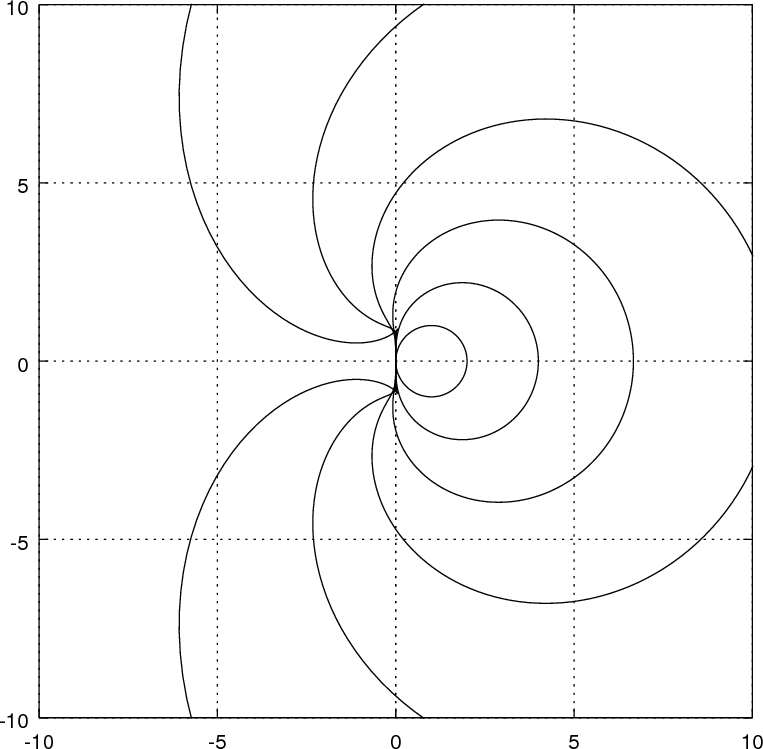
\includegraphics[width=.45\textwidth]{fig/stability-bdf.png}
  \hfill
  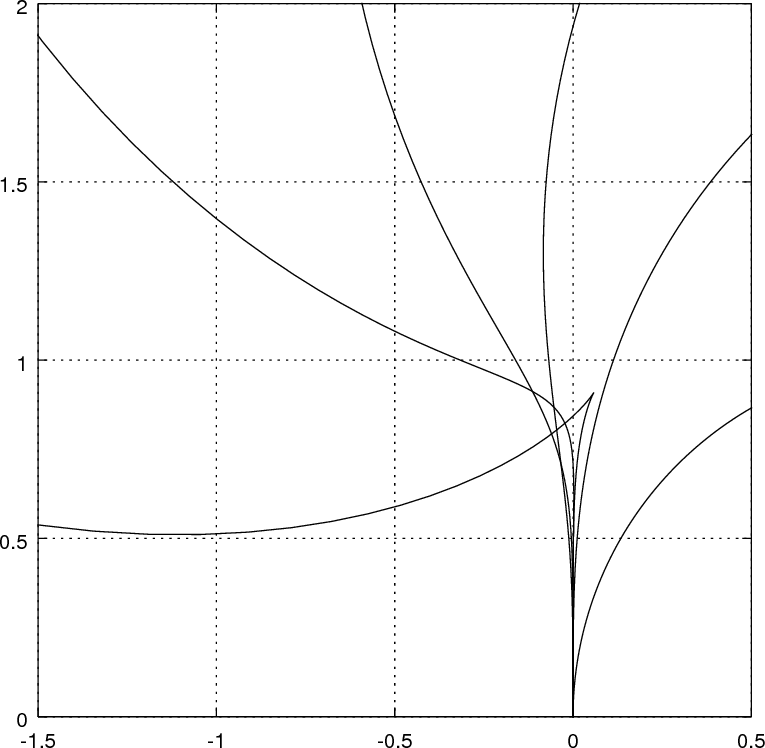
\includegraphics[width=.45\textwidth]{fig/stability-bdf-zoom.png}
  \caption{Boundaries of stability regions of BDF1 to BDF6. Unstable
    region right of the origin. Zoom on the right}
  \label{fig:bdf-stability}
\end{figure}
\begin{table}[tp]
  \centering
  \begin{tabular}{c|cccccc}
    $k$ & 1 & 2 & 3 & 4 & 5 & 6 \\\hline
    $\alpha$ & 90$^\circ$ & 90$^\circ$& 86.03$^\circ$
                    & 73.35$^\circ$& 51.84$^\circ$
                            & 17.84$^\circ$ \\
    $D$ & 0 & 0 & 0.083& 0.667& 2.327& 6.075
  \end{tabular}
  \caption{Values for A($\alpha$)- and stiff stability for BDF methods
    of order $k$.}
  \label{tab:bdf-stability}
\end{table}

%%%%%%%%%%%%%%%%%%%%%%%%%%%%%%%%%%%%%%%%%%%%%%%%%%%%%%%%%%%%%%%%%%%%%%
\section{Predictor-corrector schemes}

\begin{Definition*}{predictor-corrector}{Predictor-corrector methods}
  Assume a pair of time stepping schemes, one explicit, one implicit,
  \begin{align*}
    \hat y_{k} &= \hat \verfahren_p(y_{k-1}) \\
    y_k &= \verfahren_c(y_{k-1},y_{k}),
  \end{align*}
  we can use $\hat y_k$ as initial value for the Newton iteration for
  $y_k$. In an extreme case, we let
  \begin{gather*}
    y_k = \verfahren_c(y_{k-1},\hat y_{k}),
  \end{gather*}
  without any further iteration.
\end{Definition*}

\begin{remark}
  Predictor-corrector methods were developed strongly around
  Adams-Moulton and Adams-Bashforth methods, since the implicit ones
  have much smaller error constants. Given that these methods offer no
  considerable advantages compared to Runge-Kutta methods, but
  stability properties and implementation are weak points, We omit
  their discussion.

  A simple predictor for BDF methods can be obtained, since they are
  based on an interpolating polynomial. Thus, we simply extrapolate
  this polynomial to the next point in time.
\end{remark}

\begin{example}
  While the predictor-corrector idea sounds reasonable, we have to be
  careful with stiff problems, the original reason for using implicit
  methods. Take again our favorite IVP
  \begin{gather*}
    u' = \lambda u,
    \qquad u(0) = 1.
  \end{gather*}
  We apply the BDF(1) scheme, namely the implicit Euler method, with
  step size 1. According to its stability
  function~\eqref{eq:impl:stabil:impleuler}, we obtain
  \begin{gather*}
    y_1 = \frac1{1-\lambda}.
  \end{gather*}
  Hence, the interpolating polynomial is
  \begin{gather*}
    y(t) = (1-t) + \frac1{1-\lambda} t = 1 + \frac{\lambda}{1-\lambda}t.
  \end{gather*}
  For the mildly stiff problem $\lambda = -3$, we obtain
  \begin{gather*}
    y_1 = 0.25, \qquad y_2 = 0.0625,
    \qquad \hat y_2 = y(2) = -0.5.
  \end{gather*}
  Thus, the extrapolated value is already a much worse initial value
  for a Newton iteration than using the value from the previous time
  step.
  
  While this example was particularly chosen to exhibit such failure,
  it does show that extrapolation of stiff problems has its
  pitfalls. Here, we end up with a time step restriction which is
  comparable to the stability condition of the explicit method.
\end{example}


%%% Local Variables: 
%%% mode: latex
%%% TeX-master: "notes"
%%% End: 


\begin{remark}
  \index{step size!constant} The LMM was defined for constant step size
  $h$.  In principle it is possible to implement the method with a
  variable step size but we restrict ourselves to the constant case.
  Notes to the step size control can be found later on in this chapter.
\end{remark}

\begin{remark}
  One-step methods were always denoted by describing how to compute
  $y_1$ from $y_0$. Here, the notation becomes more complicated, but
  sometimes we consider only $y_s$ computed from $y_0,\dots,y_{s-1}$
  implying the same rules for $y_k$ computed from
  $y_{k-\lmms},\dots,y_{k-1}$.
\end{remark}
\begin{Definition}{lmm-errors}
    \index{Lh@$L_h$|textbf}
  We express the LMM with the linear \define{difference operator}
  \begin{gather}
    \label{eq:lmm:9}
    (L_hu)(t_k) = \sum_{r=0}^{\lmms}\Bigl(\alpha_{\lmms-r} u(t_{k-r}) - h
    \beta_{R-r} f\bigl(t_{k-r},u(t_{k-r})\bigr)\Bigr)
  \end{gather}
  and for a continuous function $u$ we define the \textbf{truncation
    error}\defindex{truncation error!LMM}
  \begin{gather}
    \label{eq:lmm:10}
    \tau_h(t_k) = \tfrac1hL_hu(t_k).
  \end{gather}
  The \textbf{local error} \defindex{LMM!local error}\defindex{local
    error!LMM} of a linear multistep method is defined by
  \begin{gather*}
    u(t_\lmms) - y_\lmms
  \end{gather*}
  where $u(t)$ denotes the exact solution of $u' = f(t,u), u(t_0)=u_0$
  and $y_s$ the numerical solution by using the exact initial values
 	$y_i = u(t_i)$ for $i = 0,1,...,s-1$.
\end{Definition}

%%% Local Variables:
%%% mode: latex
%%% TeX-master: "../notes"
%%% End:


\begin{lemma}
  Consider the differential equation
  \begin{gather*}
    y' = f(t,y) \qquad y(t_0) = y_0
  \end{gather*}
  where f is given continuously differentiable and $y(t)$ is the exact solution.
  For the local error we obtain

  \begin{gather}
    y(t_k)-y_k = \left( \alpha_0 \identity - h\beta_0 \frac{\partial f}{\partial y}(t_k,\eta) \right)^{-1} (L_h u)(t_k).
  \end{gather}

  Here $\eta$ is a value between $y(t_k)$ and $y_k$ if $f$ is a scalar
	function.
  If $f$ is multidimensional, the matrix 
	$\frac{\partial f}{\partial y}(t_k,\eta)$ is the Jacobi matrix, 
	which rows are evaluated at possible places between
	$y(t_k)$ and $y_k$.
\end{lemma}

\begin{proof}
  Considering the local error we can assume exact initial values 
  and therefore we can transform ~\ref{eq:lmm:4} to:
  \begin{gather*}
    \alpha_\lmms y_k + \sum\limits_{r=1}^\lmms \alpha_{\lmms-r} y(t_{k-r})
    = h \left( \beta_\lmms f_k + \sum\limits_{r=1}^\lmms \beta_{\lmms-r} f_{k-r} \right)
  \end{gather*}
  We transform further:
  \begin{multline*}
    \sum\limits_{r=0}^{\lmms} \left( \alpha_r y(t_{k-r})
      - h \beta_r f(t_{k-r},y(t_{k-r})) \right)
    \\
    - \alpha_0 y(t_k) + h \beta_0 f(t_k, y(t_k)) + \alpha_0 y_k
    - h \beta_0 f(t_k,y_k) = 0.
  \end{multline*}
	We now insert ~\ref{eq:lmm:9} which results in
  \begin{gather*}
    (L_h y)(t_k) = \alpha_0 \left( y(t_k) - y_k \right) - h \beta_0 \left( f(t_k,y(t_k)) - f(t_k,y_k) \right)
    \\
    \left( y(t_k) - y_k \right) \left( \alpha_0 \identity - h \beta_0 \frac{f(t_k,y(t_k)) - f(t_k,y_k)}{y(t_k) - y_k} \right)
  \end{gather*}
  By application of the mean value theorem and 
  subsequent transformation we obtain the statement of the theorem.
\end{proof}

      % \cite[Lemma 2.2, p. 369]{HairerNorsettWanner93}

\begin{Definition}{lmm-consistency}
  An LMM is consistent of order $p$, if for all sufficient regular
  functions $u$ and all relevant $k$ there holds
  \begin{gather}
    \label{eq:lmm:11}
    \tau_h(t_k) = \mathcal O(h^p),
  \end{gather}
  or equivalently, that the \putindex{local error} is $\mathcal O(h^{p+1})$.
\end{Definition}

%%% Local Variables:
%%% mode: latex
%%% TeX-master: "../notes"
%%% End:

\begin{Lemma}{lmm-bramble-hilbert}
  An LMM is consistent of order $p$ if and only if for all polynomials
  $\phi_q$ of degree $q \le p$ and $f(t,q(t)) = q'(t)$ there holds:
  \begin{gather}
    \label{eq:lmm:14}
    L_h \phi_q = 0.
  \end{gather}
\end{Lemma}

%%% Local Variables:
%%% mode: latex
%%% TeX-master: "../notes"
%%% End:


\begin{proof}
  We start with the Taylor expansion of a solution $u$ of the ODE and
  the corresponding right hand side $f$ for $t_k$, where we insert,
  unlike usual, $f=u'$:
  \begin{alignat*}2
    u(t) &= \sum_{i=0}^p \frac{u^{(i)}(t_k)}{i!}(t-t_k)^i +
    \frac{u^{(p+1)}(\xi)}{(p+1)!}(t-t_k)^{p+1} &=:& \phi(t) + r_u(t)
    \\
    f\bigl(t,u(t)\bigr) &= \sum_{i=1}^p \frac{u^{(i)}(t_k)}{(i-1)!}(t-t_k)^{i-1} +
    \frac{u^{(p+1)}(\xi)}{p!}(t-t_k)^{p} &=:& \phi'(t) + r_f(t),
  \end{alignat*}
  with the Taylor polynomial $\phi(t)$ of degree $p$ and remainder
  $r_u(t)$ and $r_f(t)$. Out of this we calculate:
  \begin{align*}
    L_h u(t_k) =& \sum_{r=0}^\lmms \alpha_{\lmms-r} \phi(t_{k-r}) - h
    \sum_{r=0}^\lmms \beta_{\lmms-r} \phi'(t_{k-r})
    \\
    &+ \sum_{r=0}^\lmms \alpha_{\lmms-r} r_u(t_{k-r}) - h
    \sum_{r=0}^\lmms \beta_{\lmms-r} r_f(t_{k-r}).
  \end{align*}
  Since $t_{k-r}-t_k = r h$, the first row equals a polynomial 
  $\psi(h)$ in $h$ of degree $p$. For the second row we insert the
	reminder estimate $r_u(t) = \mathcal O((t-t_k)^{p+1}) = h
  r_f(t)$ and get:
  \begin{gather}
    \label{eq:lmm:15}
    L_h u(t_k) = L_h \phi(t_k) + \mathcal O(h^{p+1}) = \psi(h) + \mathcal O(h^{p+1}).
  \end{gather}
  According to the definition of the truncation error, this term has to be of
	order $p+1$, such that the method is of order $p$. However it is $\psi$
  of degree $p$. This can only hold true if $L_h\phi=\psi\equiv
  0$. On the other hand $\tau_h(t_k)$ automatically is of order
  $p$. Since $u$ is the solution of an arbitrary right hand side, this
	condition has to be satisfied for all kind of Taylor polynomials $\phi$ 
	of degree $p$.
\end{proof}

\begin{Theorem}{lmm-consistency}
  \index{step size!constant}
  A LMM with constant step size is consistent of order
  $p$ if and only if
    \begin{gather}
      \label{eq:lmm:12}
      \begin{split}
      \sum_{r=0}^\lmms \alpha_{r} &= 0, \\
      \sum_{r=0}^\lmms \bigl(\alpha_{r}r^q - q \beta_{r}
      r^{q-1}\bigr) &= 0,
      \qquad q = 1,\dots,p        
      \end{split}
    \end{gather}
\end{Theorem}


\begin{proof}
  According to lemma~\ref{Lemma:lmm-bramble-hilbert} it is sufficient
  to show that ~\eqref{eq:lmm:12} is equivalent to $L_h \phi_q=0$ for
  polynomials of degree $q\le p$. Due to linearity of the method it
  however is sufficient to show this for a basis of the polynomial
  space of degree $p$.  For that we choose the monomial basis of the
  form
  \begin{gather*}
  \pi_q(t) =
  \left(\frac{t-t_{k-\lmms}}h\right)^q,\qquad q=0,\dots,p.
  \end{gather*}
  For those it holds: $\pi_q(t_{k-r}) = (\lmms-r)^q$. Now we see that
  the first condition is $L_h\pi_0 = 0$ (here is
  $\pi_0'\equiv0$) and the second condition is $L_h\pi_q = 0$.
\end{proof}

\begin{todo}
  Beispiel einer konsistenten LMM, die nicht konvergiert.
\end{todo}

\begin{remark}
  As shown in a homework problem, a consistent LMM is not necessary
  convergent. To understand this behavior and develop criteria for
  convergence we need to diverge into the theory of difference
  equations.
\end{remark}
%%%%%%%%%%%%%%%%%%%%%%%%%%%%%%%%%%%%%%%%%%%%%%%%%%%%%%%%%%%%%%%%%%%%%%
%%%%%%%%%%%%%%%%%%%%%%%%%%%%%%%%%%%%%%%%%%%%%%%%%%%%%%%%%%%%%%%%%%%%%%
\section{Properties of difference equations}
%%%%%%%%%%%%%%%%%%%%%%%%%%%%%%%%%%%%%%%%%%%%%%%%%%%%%%%%%%%%%%%%%%%%%%
%%%%%%%%%%%%%%%%%%%%%%%%%%%%%%%%%%%%%%%%%%%%%%%%%%%%%%%%%%%%%%%%%%%%%%

\begin{intro}
  The stability of LMM can be understood by employing the fairly old
  theory of difference equations. In order to keep the presentation
  simple in this section, we use a different notation for numbering
  indices in the equations. Nevertheless, the coefficients of the
  characteristic polynomial are the same as for LMM.
\end{intro}

\begin{Definition}{difference-equation}
  An equation of the form
  \begin{gather}
    \label{eq:lmm:3}
    \sum_{r=0}^\lmms \alpha_{r} y_{n+r} = 0
  \end{gather}
  is called a homogeneous \define{difference equation}. A sequence
  $\{y_n\}_{n=0,\dots,\infty}$ is solution of the difference equation,
  if the equation holds true for all $n\ge \lmms$. The values
  $y_n$ may be from any of the spaces $\R$, $\C$, $\R^d$ or $\C^d$.

  The \define{generating polynomial} of this difference equation
  is
  \begin{gather}
    \label{eq:lmm:2}
    \chi(x) = \sum_{r=0}^\lmms \alpha_{r} x^{r}.
  \end{gather}

\end{Definition}

%%% Local Variables:
%%% mode: latex
%%% TeX-master: "../notes"
%%% End:


\begin{Lemma}{lmm:1}
  The solutions of the equation~\eqref{eq:lmm:3} with $y_n\in \R$ or
  $y_n\in \C$ form a vector space of dimension $\lmms$. 
\end{Lemma}

\begin{proof}
  Since the equation~\eqref{eq:lmm:3} is linear and homogeneous, it is
  obvious that if two sequences of solutions $\{y^{(1)}\}$ and
  $\{y^{(2)}\}$ satisfy the equation, sums of multiples of them
  satisfy it too.

  As soon as the initial values $y_0$ to $y_{\lmms-1}$ are chosen, all
  other sequence members are uniquely defined.  Moreover it holds
  \begin{gather*}
    y_0=y_1=\dots=y_{\lmms-1}=0
    \quad\Longrightarrow\quad
    y_n = 0, \;n \ge 0.
  \end{gather*}
  Therefore it is sufficient to consider the first $\lmms$ values.  If
  they are linear independent, then the overall sequences are and vice
  versa. Thus, the initial values form a $\lmms$
  dimensional vector space.
\end{proof}

\begin{Lemma}{difference-equation-solutions}
  For each root $\xi$ of the generating polynomial $\chi(x)$ the
  sequence $y_n = \xi^n$ is a solution of the difference
  equation~\eqref{eq:lmm:3}.
\end{Lemma}


%%% Local Variables: 
%%% mode: latex
%%% TeX-master: "../notes"
%%% End: 


\begin{proof}
  Inserting the solution $y_n = \xi^n$ into the difference equation
  results in
  \begin{gather*}
    \sum_{r=0}^\lmms \alpha_{r} \xi^{n+r} = \xi^{n}
    \sum_{r=0}^\lmms \alpha_{r} \xi^{r}
    = \xi^{n} \chi(\xi) = 0.
  \end{gather*}
\end{proof}

\begin{Theorem}{difference-equation-basis}
  Let $\{\xi_i\}_{i=1,\dots,\iota}$ be the roots of the
  generating polynomial $\chi$ with multiplicity $\nu_i$. Then,
  the sequences of the form
  \begin{gather}
    \label{eq:lmm:6}
%    y^{(i,k)}_n = p_k(n)\xi_i^n
    y^{(i,k)}_n = n^{k-1}\xi_i^n
    \quad i=1,\dots,\iota; \quad k = 1,\dots,\nu_i
  \end{gather}
%  mit den Polynomen
%  \begin{gather*}
%    p_0(n) = 1 \quad p_k(n) = \prod_{\kappa=0}^{k-1} (n-\kappa)
%  \end{gather*}
  form a basis of the solution space of the difference
  equation~\eqref{eq:lmm:3}.
\end{Theorem}


%%% Local Variables: 
%%% mode: latex
%%% TeX-master: "../notes"
%%% End: 


\begin{proof}
  First we observe that the sum of the multiplicities of the roots
  results in the degree of the polynomial:
  \begin{gather*}
    \lmms = \sum_{i=1}^\iota \nu_i.
  \end{gather*}
  Moreover we know because of Lemma~\ref{Lemma:lmm:1}, that $\lmms$ is
  the dimension of the solution space. We show that the sequences
  $\{y^{(i,k)}_n\}$ are linear independent. This is clear for
  sequences of different index $i$. It is also clear for different roots,
  because for $n\to\infty$ the exponential function nullifies the
  influence of the polynomials.
  
  It remains to show that the sequences $\{y^{(i,k)}_n\}$ in fact are
  solutions of the difference equations.  For $k=0$ we have proven
  this already in lemma~\ref{Lemma:difference-equation-solutions}.  We proof the fact here for
  $k=2$ and for a double zero $\xi_i$; the principle for higher order
  roots should be clear then.  Equation~\eqref{eq:lmm:3} applied to
  the sequence $\{n \xi_i^n\}$ results in
  \begin{align*}
    \sum_{r=0}^{\lmms} \alpha_r (n+r) \xi_i^{n+r}
    &= n \xi_i^n \sum_{r=0}^{\lmms} \alpha_r \xi_i^{r}
    + \xi_i^{n+1} \sum_{r=1}^{\lmms} \alpha_r r \xi_i^{r-1}
    \\
    &= n \xi_i^n \rho(\xi_i) + \xi_i^{n+1} \rho'(\xi_i) = 0.
  \end{align*}
  Here the term with $\alpha_0$ vanishes, because it is multiplied
  with $r=0$. $\rho(\xi_i) = \rho'(\xi_i) = 0$ because $\xi_i$ is a
  multiple root.
\end{proof}

\begin{Corollary*}{root-test}{Root test}
  All solutions $\{y_n\}$ of the difference equation~\eqref{eq:lmm:3}
  are bounded for $n\to\infty$ if and only if it holds:
  \begin{itemize}
  \item all roots of the generating polynomial $\chi(x)$
    lie in the closed unit circle $\bigl\{z\in \C \big|\; |z|\le
    1\bigr\}$ and
  \item all roots on the boundary of the unit circle are simple.
  \end{itemize}
\end{Corollary*}

%%% Local Variables: 
%%% mode: latex
%%% TeX-master: "../notes"
%%% End: 


\begin{proof}
  According to theorem~\ref{Theorem:difference-equation-basis} we can write all solutions
  as linear combinations of the sequences $y^{(i,k)}$ in
  equation~\eqref{eq:lmm:6}. Therefore,
  \begin{enumerate}
  \item all solutions to $|\xi_i|<1$ for $n\to\infty$ converge to zero
  \item all solutions to $|\xi_i|>1$ for $n\to\infty$ divergence to infinity
  \item all solutions to $|\xi_i|=1$ for $n\to\infty$ stay bounded 
	if and only if $\xi_i$ is simple.
  \end{enumerate}
  This proves the statement of the theorem.
\end{proof}

%%%%%%%%%%%%%%%%%%%%%%%%%%%%%%%%%%%%%%%%%%%%%%%%%%%%%%%%%%%%%%%%%%%%%%
%%%%%%%%%%%%%%%%%%%%%%%%%%%%%%%%%%%%%%%%%%%%%%%%%%%%%%%%%%%%%%%%%%%%%%
\section{Stability and convergence}
%%%%%%%%%%%%%%%%%%%%%%%%%%%%%%%%%%%%%%%%%%%%%%%%%%%%%%%%%%%%%%%%%%%%%%
%%%%%%%%%%%%%%%%%%%%%%%%%%%%%%%%%%%%%%%%%%%%%%%%%%%%%%%%%%%%%%%%%%%%%%

\begin{remark}
  In contrast to one-step methods the convergence of multistep methods
  follows not directly from the consistency of the method, if the
  right hand side of the differential equation satisfies the Lipschitz
  condition~\eqref{eq:IVP:1}.  Analog to the A-stability we will
  discuss this by means of a simple model problem and we will deduce
  stability conditions.
\end{remark}

\begin{remark}
  In the following we investigate the solution to a fixed point in time
  $t$ with a shrinking step size $h$. Therefore we choose $n$
  steps of step size $h = t/n$ and let $n$ go towards infinity.
\end{remark}

\begin{Theorem}{lmm-stability}
  A LMM is stable if and only if all roots of the first
  generating polynomial $\rho(x)$ of equation~\eqref{eq:lmm:5} lie
  in the unit circle of the complex plane and all roots on the
  boundary of the unit circle are simple.
\end{Theorem}


%%% Local Variables: 
%%% mode: latex
%%% TeX-master: "../notes"
%%% End: 

\begin{Theorem}{lmm-stability}
  A LMM is stable if and only if all roots of the first
  generating polynomial $\rho(x)$ of equation~\eqref{eq:lmm:5} lie
  in the unit circle of the complex plane and all roots on the
  boundary of the unit circle are simple.
\end{Theorem}


%%% Local Variables: 
%%% mode: latex
%%% TeX-master: "../notes"
%%% End: 


\begin{proof}
  The application of the LMM to the equation~\eqref{eq:lmm:1} results
  in the difference equation
  \begin{gather*}
    \sum_{r=0}^{\lmms} \alpha_{\lmms-r} y_{n-r} = 0.
  \end{gather*}
  Now we have to proof that the solutions for fixed $t = h n$ stay
  bounded if $h\to 0$. But we also see that the upper equation does
  not contain $h$. Therefore we have to examine, if the solutions
  $y_n$ stay bounded for $n\to \infty$.  By resorting the summation we
  obtain a difference equation of the form~\eqref{eq:lmm:3}. Due to
  corollary~\ref{Corollary:root-test} it follows the statement of the theorem.
\end{proof}

\begin{Corollary}{adams-stability}
  Adams-Bashforth and Adams-Moulton methods are stable.
\end{Corollary}

\begin{proof}
  For all of these methods the first generating polynomial is $\rho(x)
  = x^\lmms-x^{\lmms-1}$. It has the simple root $\xi_1 = 1$ and the
  $\lmms-1$-fold root 0.
\end{proof}

\begin{Theorem}{BDF-stability}
  The BDF methods are stable for $\lmms \le 6$ and not
  stable for $\lmms \ge 7$.
\end{Theorem}

\begin{Theorem}{lmm-convergence}
  If a linear multi-step method is stable and consistent of order $p$,
  then it is convergent of order $p$.
\end{Theorem}

%%% Local Variables: 
%%% mode: latex
%%% TeX-master: "../notes"
%%% End: 

\begin{Lemma}{lmm-one-step}
  Every multistep method can be recast as a one-step method
  \begin{gather}
    \label{eq:lmm-one-step:1}
    Y_{k} = (A \otimes \identity) Y_{k-1} + h \verfahren_h(t_{k-1}, Y_{k-1})
  \end{gather}
  where with $\alpha_r' = \alpha_r/\alpha_s$
  \begin{gather}
    \label{eq:lmm-one-step:2}
    Y_k =
    \begin{pmatrix}
      y_k \\ \vdots \\ y_{k-s+1}
    \end{pmatrix},
    \quad
    A =
    \begin{pmatrix}
      -\alpha_{\lmms-1}' & -\alpha_{\lmms-2}' & \cdots & -\alpha_{0}'\\
      1 & 0 & \cdots & 0 \\
      & \ddots & \cdots & 0 \\
      & & 1 & 0
    \end{pmatrix},
  \end{gather}
  and $\verfahren_h(t_k, Y_k) = (e_1 \otimes \identity) \psi_h(t_{k-1}, Y_{k-1})$ with
  $\beta_r' = \beta_r/\alpha_s$ and $\psi_h$ defined implicitly by
  \begin{multline}
    \label{eq:lmm-one-step:3}
    \psi_h(t_{k-1}, Y_{k-1})
    =\sum_{r=1}^{\lmms} \beta_{\lmms-r} f(t_{k-r},y_{k-r})
    \\
    + \beta_s' f\left(t_k, h\psi_h(t_{k-1}, Y_{k-1}) -
      \sum_{r=1}^{\lmms} \alpha_{\lmms-r}' y_{k-r}\right).
  \end{multline}
\end{Lemma}

%%% Local Variables: 
%%% mode: latex
%%% TeX-master: "../notes"
%%% End: 


\begin{proof}
  From the general form of LMM we
  obtain
  \begin{gather*}
    \frac1{\alpha_s} \sum_{r=0}^\lmms \alpha_{\lmms-r} y_{k-r}
    = \frac{h}{\alpha_s} \sum_{r=0}^{\lmms-1} \beta_{\lmms-r} f_{k-r}
    + \beta_s f_k.
  \end{gather*}
  We rewrite this to
  \begin{gather*}
    y_k = -\sum_{r=1}^{\lmms} \alpha'_{\lmms-r} y_{k-r} +
    h\psi_h(t_{k-1}, Y_{k-1}),
  \end{gather*}
  where we implicitly enter this formula as value for $y_k$ in the
  computation of $f_k$. It remains to realize that this is the first
  set of $d$ equations in~\eqref{eq:lmm-one-step:1}, and that the
  remaining ones are just shifting $y_i$ to $y_{i+1}$.
\end{proof}

\begin{Lemma}{lmm-one-consistency}
  Let $u(t)$ be the exact solution of the IVP. For $k=s,\ldots$, we
  define the vector $\widehat Y_{k}$ as the solution of a single step
  \begin{gather*}
    \widehat Y_{k} = (A\otimes I) U_{k-1} + h \verfahren_h(t_{k-1} U_{k-1}),
  \end{gather*}
  with correct initial values $U_{k-1} =
  (u_{k-1},u_{k-2},\dots,u_{k-\lmms})^T$.
  
  If the multistep method is consistent of order $p$, and $f$ is
  sufficiently smooth, then there exist constants $h_0>0$  and $M$
  such that for $h\le h_0$ there holds
  \begin{gather}
    \label{eq:lmm-one-consistency:1}
    \norm{Y_k-\widehat Y_h} \le M h^{p+1}.
  \end{gather}
\end{Lemma}

%%% Local Variables: 
%%% mode: latex
%%% TeX-master: "../notes"
%%% End: 


\begin{proof}
  The first component of $Y_k - \widehat Y_k$ is the local error of
  step $k$, which is of order $h^{p+1}$ by the assumption. The other
  components vanish by the definition of the method.
\end{proof}

\begin{Lemma}{lmm-one-stability}
  Assume that an LMM is stable. Then, there exists a vector norm on
  $\C^{\lmms d}$ such that the operator norm of the matrix $A$
  satisfies
  \begin{gather}
    \label{eq:lmm-one-stability:1}
    \norm{A\otimes \identity} \le 1.
  \end{gather}
\end{Lemma}

%%% Local Variables: 
%%% mode: latex
%%% TeX-master: "../notes"
%%% End: 


\begin{proof}
  We notice that $\widehat\rho(x) = \sum \alpha'_{s-r} x^r$ is the
  characteristic polynomial of the matrix $A$ and thus its eigenvalues
  are the roots of $\widehat\rho(x)$, which has the same roots as the
  generating polynomial $\rho(x)$. By the root test, we know that
  simple roots, which correspond to irreducible blocks of dimension
  one have maximal modulus one. Furthermore, every Jordan block of
  dimension greater than one corresponds to a multiple root, which by
  assumption has modulus strictly less than one. It is easy to see
  that such a block admits a modified canonical form
  \begin{gather*}
    J_i =
    \begin{pmatrix}
      \lambda_i & 1- \abs{\lambda_i}\\
        & \lambda_i &\ddots\\
          &&\ddots & 1- \abs{\lambda_i}\\
            &&&\lambda_i
    \end{pmatrix}.
  \end{gather*}
  Thus, the canonical form $J = T^{-1}AT$ has norm $\norm{J}_{\infty}
  \le 1$. If we define the norm
  \begin{gather*}
    \norm{x} = \norm{(T^{-1}\otimes \identity)x}_\infty,
  \end{gather*}
  we obtain the result by
  \begin{multline*}
    \norm{(A\otimes \identity)x}
    = \norm{(T^{-1}\otimes \identity)(A\otimes \identity)x}_\infty
    = \norm{(J\otimes \identity)(T^{-1}\otimes \identity)x}_\infty
    \\
    \le \norm{(T^{-1}\otimes \identity)x}_\infty
    = \norm{x}.
  \end{multline*}
\end{proof}

\begin{Theorem}{lmm-convergence}
  If a linear multi-step method is stable and consistent of order $p$,
  then it is convergent of order $p$.
\end{Theorem}

%%% Local Variables: 
%%% mode: latex
%%% TeX-master: "../notes"
%%% End: 


\begin{proof}
  We reduce the proof to convergence of a one-step method with
  \begin{gather}
    \label{eq:lmm:18}
    Y_k = G(Y_{k-1}) =  (A\otimes \identity) Y_{k-1} + h \verfahren_h(t_{k-1}, Y_{k-1}).
  \end{gather}
  Let $Y_{k-1}$ and $Z_{k-1}$ be two initial values for the interval $I_k$.
  By the previous lemma, we have in the norm defined there, for
  sufficiently small $h$, and assuming a Lipschitz constant $L_h$ for
  $\verfahren_h$ :
  \begin{gather}
    \label{eq:lmm:19}
    \norm{G(Y_{k-1})-G(Z_{k-1})} \le (1+h L_h) \norm{Y_{k-1}-Z_{k-1}}.
  \end{gather}
  Thus, the local error $\eta_k = U_k - \widehat Y_k$ at step $k$, which by
  Lemma~\ref{Lemma:lmm-one-consistency} is bounded by $M h^{p+1}$, accumulates
  until step $n$ at most to $h^{p+1}(1_h L_h)^{n-k}$.

  We have:
  \begin{align*}
    \norm{U_1 - Y_1} &\le (1+h L_h)\norm{U_0-y_0} + M h^{p+1} \\
    \norm{U_2 - Y_2} &\le (1+h L_h)^2\norm{U_0-y_0} +  M h^{p+1} \bigl(1+ (1+h L_h)\bigr)\\
    \norm{U_3 - Y_3} &\le (1+h L_h)^3\norm{U_0-y_0} +  M h^{p+1} \Bigl(\bigl(1+ (1+h L_h)+ (1+h L_h)^2\bigr)\Bigr)\\
    \norm{U_n-Y_n} &\le e^{n h L_h}\norm{U_0-Y_0} +
    \frac{M h^p}{L_h}\bigl(e^{n h L_h} - 1\bigr).
  \end{align*}
\end{proof}

\subsection{Starting procedures}

\begin{intro}
In contrast to one-step methods, where the numerical solution is obtained 
solely from the differential equation and the initial value, multistep 
methods require more than one start value. An LMM with $s$ steps requires $s$ 
known start values $y_{k-s}, \dots, y_{k-1}$. Mostly, they are not provided 
by the IVP itself. Thus, general LMM decompose into two parts: 
\begin{itemize}
\item a \emph{starting phase} where the start values are computed in a 
suitable way and
\item a \emph{run phase} where the LMM is executed. 
\end{itemize}
It is crucial that the method of the starting phase provides a suitable order 
corresponding to the LMM of the run phase, recall Definition 
\ref{Definition:lmm-convergence}. Moreover, it should have analog properties to 
the LMM, like explicit/implicit or applicability to stiff problems. 
% We now consider different starting procedures for an implicit LMM with 
% convergence order $p$. According to Definition \ref{Definition:lmm-convergence} 
% the starting values are required to have the same convergence order. 
Possible choices for the starting phase include multistep methods with variable 
order and one-step methods.  
\end{intro}

\begin{example}[Self starter]
A 2-step BDF method requires $y_0$ and $y_1$ to be known. $y_0$ is given by the 
initial value while $y_1$ is unknown so far. To guarantee that the method has 
order 2, $y_1$ needs to be locally of order 2 at least
\begin{align}\label{eq:lmm_1BDFstarter}
|u(t_1)-y_1| \leq c_0 h^2.
\end{align}
This is ensured, for example, by one step of the 1-step BDF method.

However, starting an LMM with $s>2$ steps by a first-order method and then 
successively increasing the order until $s$ is reached does not provide the 
desired global order. That is due to the fact that the first step limits  
the overall convergence order to 2, compare \eqref{eq:lmm_1BDFstarter}. 
Nevertheless, self starters are often used in practice. 
\end{example}
% In this case local 
% error estimates are used to bound the errors of the starting values and all 
% approximations of the run phase by reducing the step sizes, 
% %. Moreover, also in 
% %the run phase the step sizes are controlled using local error estimates, 
% see the  
% discussion on step size control in Section \ref{section:step_size_control}. 


\begin{example}[Runge-Kutta starter]
\label{Example:RKstarter}
One can use Runge-Kutta methods to start LMM. Since only a fixed
number of starting steps are performed, the local order of the
Runge-Kutta approximation is crucial.  For an implicit LMM with
convergence order $p$ and stepsize $h$ one could use an RK method with
consistency order $p-1$ with the same stepsize $h$.

Consider a 3-step BDF method. Thus, beside $y_0$, we need start values 
$y_1, y_2$ with errors less than $c_0 h^3$. They can be computed by RK methods 
of consistency order $2$, for example by two steps of the 1-stage Gau\ss \ 
collocation method with step size $h$ since it has consistency order $2s=2$, 
see theorem \ref{Theorem:gauss-consistency}.
\end{example}




\begin{example}[Continuous Runge-Kutta starter]
  Another option is to use continuous Runge-Kutta methods and to
  evaluate the continuous approximation to obtain the required
  starting values.

  In constrast to Example \ref{Example:RKstarter} one could also use
  the continuous polynomial approximation of Gau\ss \ collocation to
  start a 3-step BDF method. One step with step size $2h$ of a 2-stage
  Gau\ss \ collocation method would give a polynomial of degree $2$
  which is then evaluated in $t_1=t_0+h$ and $t_2=t_1+h$ to obtain
  $y_1, y_2$. According to Theorem
  \ref{Theorem:collocation-continuous} $y_1, y_2$ have the appropriate
  order.
\end{example}

\begin{remark}
  In practice not the order of a procedure is crucial but rather the
  fact that the errors of all approximations (the start values and all
  approximations of the run phase) are bounded by the user-given
  tolerance, compare Section \ref{section:step_size_control}. Thus,
  the step sizes of all steps are controlled using local error
  estimates. Hence, self starting procedures usually start with very
  small step sizes and increase them successively. Due to their higher
  orders RK starters usually are allowed to use moderate step sizes in
  the beginning. Generally, LMM are applied with variable step sizes
  and orders in practice (see e.g. Exercise 7.2).
\end{remark}



%%%%%%%%%%%%%%%%%%%%%%%%%%%%%%%%%%%%%%%%%%%%%%%%%%%%%%%%%%%%%%%%%%%%%%
%%%%%%%%%%%%%%%%%%%%%%%%%%%%%%%%%%%%%%%%%%%%%%%%%%%%%%%%%%%%%%%%%%%%%%
\section{LMM and stiff problems}
%%%%%%%%%%%%%%%%%%%%%%%%%%%%%%%%%%%%%%%%%%%%%%%%%%%%%%%%%%%%%%%%%%%%%%
%%%%%%%%%%%%%%%%%%%%%%%%%%%%%%%%%%%%%%%%%%%%%%%%%%%%%%%%%%%%%%%%%%%%%%

\begin{Definition*}{lmm-stability-region}{A-stability of LMM}
  \index{stability region!of a LMM}
  The linear model difference equation
  \begin{gather}
    \label{eq:lmm:7}
    \sum_{r=0}^{\lmms} \bigl(\alpha_{\lmms-r} - z \beta_{\lmms-r}) y_{n-r} = 0.
  \end{gather}
  is obtained by applying an LMM to the model equation
  $u' = \lambda u$ and inserting $z=h\lambda$.

  The \define{stability region} of an LMM is the set of points $z\in \C$,
  for which all solution sequences $\{y_n\}$ of the equation~\eqref{eq:lmm:7}
  stay bounded for $n\to\infty$. An LMM is called \define{A-stable}, if the 
  stability region contains the left half-plane of $\C$.
\end{Definition*}


\begin{Definition}{lmm-stability-polynomial}
  The stability polynomial of an LMM is obtained by inserting
  $y_n = x^n$ into the linear model difference equation to obtain
  \begin{gather}
    \label{eq:lmm:8}
    r_z(x) = \sum_{r=0}^{\lmms} \bigl(\alpha_{\lmms-r} - z \beta_{\lmms-r})
    x^{\lmms-r}.
  \end{gather}
\end{Definition}

\begin{remark}
  Instead of the simple amplification function $r(z)$ of the one-step
  methods, we get here a function of two variables.  The point $z$ for
  which we want to show stability and the artificial variable $x$ from
  the analysis of the method.
\end{remark}

\begin{Lemma}{lmm-stability}
  Let $\{\xi_1(z),\dots,\xi_\lmms(z)\}$ be the set of roots of the
  stability polynomial $r_z(x)$ as functions of $z$.
  A point $z\in \C$ is in the stability region of a LMM, if these
  roots satisfy the root test in corollary~\ref{Corollary:root-test}.
\end{Lemma}

\begin{proof}
  The proof is analog to theorem~\ref{Theorem:lmm-stability}.
\end{proof}

\begin{Theorem*}{dahlquist2}{2nd Dahlquist barrier}
  \defindex{Dahlquist barrier (second)} There is no A-stable LMM of
  order $p>2$. Among the A-stable LMM of order 2, the trapezoidal rule
  (Crank-Nicolson) has the smallest error constant.
\end{Theorem*}

\subsection{Relaxed A-stability}

\begin{intro}
  Motivated by the fact that there are no higher order A-stable LMM
  and by highly dissipative problems, people have introduced relaxed
  concepts of A-stability.
\end{intro}

\begin{Definition}{aa-stability}
  \defindex{A($\alpha$)-stable}
  A set is called \textbf{A($\alpha$)-stable}, if its stability region
  contains the sector
  \begin{gather*}
    \bigg\{z\in \C\;\bigg|\; \Re z < 0 \;\wedge\; \left|\frac{\Im
        z}{\Re z}\right| \le \tan \alpha\biggr\}.
  \end{gather*}
  It is called \textbf{A(0)-stable}, if the negative real axis is contained in
  the stability region.

  It is called \define{stiffly stable}, if it contains the set
  $\{\Re(z)< -D\}$.
\end{Definition}

%%% Local Variables:
%%% mode: latex
%%% TeX-master: "../notes"
%%% End:


\begin{remark}
  The introduction of the A(0)-stability is motivated by linear
  systems of the form $u'=-Au$ with symmetric, positive definite
  matrix $A$. In fact one requires there only stability on the real
  axis because all eigenvalues are real. Thus, any positive angle
  $\alpha$ is sufficient.
  
  Similarly A($\alpha$)-stable LMM are suitable for linear problems in
  which high frequently vibration ($\Im\lambda$ large) decay fast
  ($-\Re\lambda$ large).

  In all cases one observes corresponding properties of the Jacobian
  matrix $\partial_u f$ for the application of nonlinear problems.
\end{remark}

\begin{example}
  The stability regions of the stable BDF methods are in
  Figure~\ref{fig:bdf-stability}. The corresponding values for
  A($\alpha$)-stability and stiff stability are in Table  
\ref{tab:bdf-stability}.
\end{example}
\begin{figure}[tp]
  \centering
  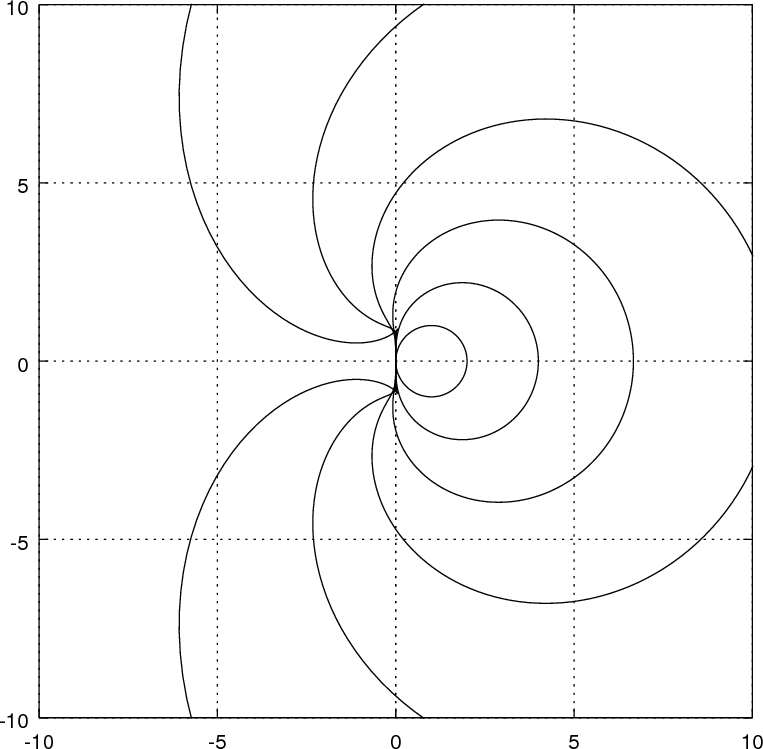
\includegraphics[width=.45\textwidth]{fig/stability-bdf.png}
  \hfill
  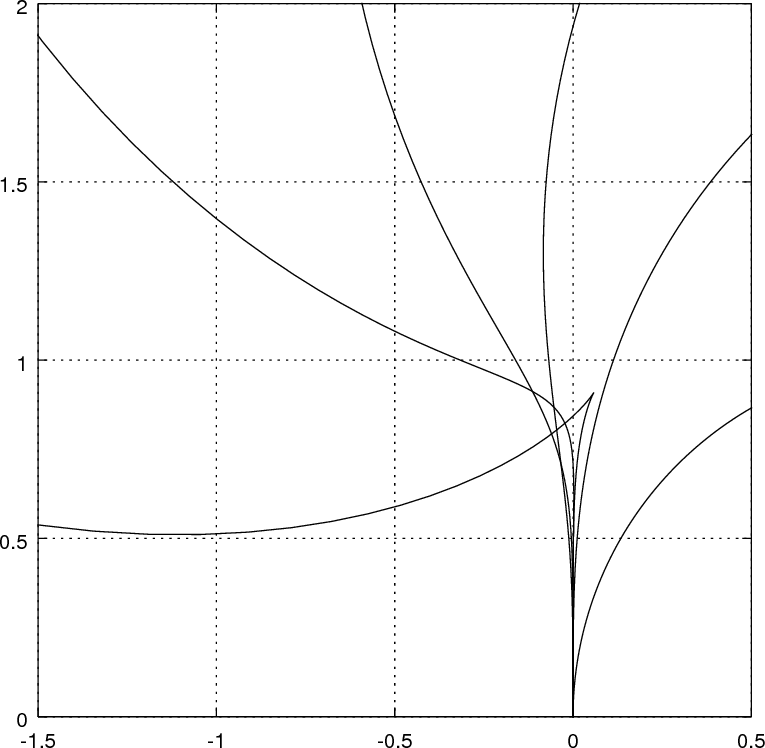
\includegraphics[width=.45\textwidth]{fig/stability-bdf-zoom.png}
  \caption{Boundaries of stability regions of BDF1 to BDF6. Unstable
    region right of the origin. Zoom on the right}
  \label{fig:bdf-stability}
\end{figure}
\begin{table}[tp]
  \centering
  \begin{tabular}{c|cccccc}
    $k$ & 1 & 2 & 3 & 4 & 5 & 6 \\\hline
    $\alpha$ & 90$^\circ$ & 90$^\circ$& 86.03$^\circ$
                    & 73.35$^\circ$& 51.84$^\circ$
                            & 17.84$^\circ$ \\
    $D$ & 0 & 0 & 0.083& 0.667& 2.327& 6.075
  \end{tabular}
  \caption{Values for A($\alpha$)- and stiff stability for BDF methods
    of order $k$.}
  \label{tab:bdf-stability}
\end{table}

%%%%%%%%%%%%%%%%%%%%%%%%%%%%%%%%%%%%%%%%%%%%%%%%%%%%%%%%%%%%%%%%%%%%%%
\section{Predictor-corrector schemes}

\begin{Definition*}{predictor-corrector}{Predictor-corrector methods}
  Assume a pair of time stepping schemes, one explicit, one implicit,
  \begin{align*}
    \hat y_{k} &= \hat \verfahren_p(y_{k-1}) \\
    y_k &= \verfahren_c(y_{k-1},y_{k}),
  \end{align*}
  we can use $\hat y_k$ as initial value for the Newton iteration for
  $y_k$. In an extreme case, we let
  \begin{gather*}
    y_k = \verfahren_c(y_{k-1},\hat y_{k}),
  \end{gather*}
  without any further iteration.
\end{Definition*}

\begin{remark}
  Predictor-corrector methods were developed strongly around
  Adams-Moulton and Adams-Bashforth methods, since the implicit ones
  have much smaller error constants. Given that these methods offer no
  considerable advantages compared to Runge-Kutta methods, but
  stability properties and implementation are weak points, We omit
  their discussion.

  A simple predictor for BDF methods can be obtained, since they are
  based on an interpolating polynomial. Thus, we simply extrapolate
  this polynomial to the next point in time.
\end{remark}

\begin{example}
  While the predictor-corrector idea sounds reasonable, we have to be
  careful with stiff problems, the original reason for using implicit
  methods. Take again our favorite IVP
  \begin{gather*}
    u' = \lambda u,
    \qquad u(0) = 1.
  \end{gather*}
  We apply the BDF(1) scheme, namely the implicit Euler method, with
  step size 1. According to its stability
  function~\eqref{eq:impl:stabil:impleuler}, we obtain
  \begin{gather*}
    y_1 = \frac1{1-\lambda}.
  \end{gather*}
  Hence, the interpolating polynomial is
  \begin{gather*}
    y(t) = (1-t) + \frac1{1-\lambda} t = 1 + \frac{\lambda}{1-\lambda}t.
  \end{gather*}
  For the mildly stiff problem $\lambda = -3$, we obtain
  \begin{gather*}
    y_1 = 0.25, \qquad y_2 = 0.0625,
    \qquad \hat y_2 = y(2) = -0.5.
  \end{gather*}
  Thus, the extrapolated value is already a much worse initial value
  for a Newton iteration than using the value from the previous time
  step.
  
  While this example was particularly chosen to exhibit such failure,
  it does show that extrapolation of stiff problems has its
  pitfalls. Here, we end up with a time step restriction which is
  comparable to the stability condition of the explicit method.
\end{example}


%%% Local Variables: 
%%% mode: latex
%%% TeX-master: "notes"
%%% End: 


\begin{remark}
  \index{step size!constant} The LMM was defined for constant step size
  $h$.  In principle it is possible to implement the method with a
  variable step size but we restrict ourselves to the constant case.
  Notes to the step size control can be found later on in this chapter.
\end{remark}

\begin{remark}
  One-step methods were always denoted by describing how to compute
  $y_1$ from $y_0$. Here, the notation becomes more complicated, but
  sometimes we consider only $y_s$ computed from $y_0,\dots,y_{s-1}$
  implying the same rules for $y_k$ computed from
  $y_{k-\lmms},\dots,y_{k-1}$.
\end{remark}
\begin{Definition}{lmm-errors}
    \index{Lh@$L_h$|textbf}
  We express the LMM with the linear \define{difference operator}
  \begin{gather}
    \label{eq:lmm:9}
    (L_hu)(t_k) = \sum_{r=0}^{\lmms}\Bigl(\alpha_{\lmms-r} u(t_{k-r}) - h
    \beta_{R-r} f\bigl(t_{k-r},u(t_{k-r})\bigr)\Bigr)
  \end{gather}
  and for a continuous function $u$ we define the \textbf{truncation
    error}\defindex{truncation error!LMM}
  \begin{gather}
    \label{eq:lmm:10}
    \tau_h(t_k) = \tfrac1hL_hu(t_k).
  \end{gather}
  The \textbf{local error} \defindex{LMM!local error}\defindex{local
    error!LMM} of a linear multistep method is defined by
  \begin{gather*}
    u(t_\lmms) - y_\lmms
  \end{gather*}
  where $u(t)$ denotes the exact solution of $u' = f(t,u), u(t_0)=u_0$
  and $y_s$ the numerical solution by using the exact initial values
 	$y_i = u(t_i)$ for $i = 0,1,...,s-1$.
\end{Definition}

%%% Local Variables:
%%% mode: latex
%%% TeX-master: "../notes"
%%% End:


\begin{lemma}
  Consider the differential equation
  \begin{gather*}
    y' = f(t,y) \qquad y(t_0) = y_0
  \end{gather*}
  where f is given continuously differentiable and $y(t)$ is the exact solution.
  For the local error we obtain

  \begin{gather}
    y(t_k)-y_k = \left( \alpha_0 \identity - h\beta_0 \frac{\partial f}{\partial y}(t_k,\eta) \right)^{-1} (L_h u)(t_k).
  \end{gather}

  Here $\eta$ is a value between $y(t_k)$ and $y_k$ if $f$ is a scalar
	function.
  If $f$ is multidimensional, the matrix 
	$\frac{\partial f}{\partial y}(t_k,\eta)$ is the Jacobi matrix, 
	which rows are evaluated at possible places between
	$y(t_k)$ and $y_k$.
\end{lemma}

\begin{proof}
  Considering the local error we can assume exact initial values 
  and therefore we can transform ~\ref{eq:lmm:4} to:
  \begin{gather*}
    \alpha_\lmms y_k + \sum\limits_{r=1}^\lmms \alpha_{\lmms-r} y(t_{k-r})
    = h \left( \beta_\lmms f_k + \sum\limits_{r=1}^\lmms \beta_{\lmms-r} f_{k-r} \right)
  \end{gather*}
  We transform further:
  \begin{multline*}
    \sum\limits_{r=0}^{\lmms} \left( \alpha_r y(t_{k-r})
      - h \beta_r f(t_{k-r},y(t_{k-r})) \right)
    \\
    - \alpha_0 y(t_k) + h \beta_0 f(t_k, y(t_k)) + \alpha_0 y_k
    - h \beta_0 f(t_k,y_k) = 0.
  \end{multline*}
	We now insert ~\ref{eq:lmm:9} which results in
  \begin{gather*}
    (L_h y)(t_k) = \alpha_0 \left( y(t_k) - y_k \right) - h \beta_0 \left( f(t_k,y(t_k)) - f(t_k,y_k) \right)
    \\
    \left( y(t_k) - y_k \right) \left( \alpha_0 \identity - h \beta_0 \frac{f(t_k,y(t_k)) - f(t_k,y_k)}{y(t_k) - y_k} \right)
  \end{gather*}
  By application of the mean value theorem and 
  subsequent transformation we obtain the statement of the theorem.
\end{proof}

      % \cite[Lemma 2.2, p. 369]{HairerNorsettWanner93}

\begin{Definition}{lmm-consistency}
  An LMM is consistent of order $p$, if for all sufficient regular
  functions $u$ and all relevant $k$ there holds
  \begin{gather}
    \label{eq:lmm:11}
    \tau_h(t_k) = \mathcal O(h^p),
  \end{gather}
  or equivalently, that the \putindex{local error} is $\mathcal O(h^{p+1})$.
\end{Definition}

%%% Local Variables:
%%% mode: latex
%%% TeX-master: "../notes"
%%% End:

\begin{Lemma}{lmm-bramble-hilbert}
  An LMM is consistent of order $p$ if and only if for all polynomials
  $\phi_q$ of degree $q \le p$ and $f(t,q(t)) = q'(t)$ there holds:
  \begin{gather}
    \label{eq:lmm:14}
    L_h \phi_q = 0.
  \end{gather}
\end{Lemma}

%%% Local Variables:
%%% mode: latex
%%% TeX-master: "../notes"
%%% End:


\begin{proof}
  We start with the Taylor expansion of a solution $u$ of the ODE and
  the corresponding right hand side $f$ for $t_k$, where we insert,
  unlike usual, $f=u'$:
  \begin{alignat*}2
    u(t) &= \sum_{i=0}^p \frac{u^{(i)}(t_k)}{i!}(t-t_k)^i +
    \frac{u^{(p+1)}(\xi)}{(p+1)!}(t-t_k)^{p+1} &=:& \phi(t) + r_u(t)
    \\
    f\bigl(t,u(t)\bigr) &= \sum_{i=1}^p \frac{u^{(i)}(t_k)}{(i-1)!}(t-t_k)^{i-1} +
    \frac{u^{(p+1)}(\xi)}{p!}(t-t_k)^{p} &=:& \phi'(t) + r_f(t),
  \end{alignat*}
  with the Taylor polynomial $\phi(t)$ of degree $p$ and remainder
  $r_u(t)$ and $r_f(t)$. Out of this we calculate:
  \begin{align*}
    L_h u(t_k) =& \sum_{r=0}^\lmms \alpha_{\lmms-r} \phi(t_{k-r}) - h
    \sum_{r=0}^\lmms \beta_{\lmms-r} \phi'(t_{k-r})
    \\
    &+ \sum_{r=0}^\lmms \alpha_{\lmms-r} r_u(t_{k-r}) - h
    \sum_{r=0}^\lmms \beta_{\lmms-r} r_f(t_{k-r}).
  \end{align*}
  Since $t_{k-r}-t_k = r h$, the first row equals a polynomial 
  $\psi(h)$ in $h$ of degree $p$. For the second row we insert the
	reminder estimate $r_u(t) = \mathcal O((t-t_k)^{p+1}) = h
  r_f(t)$ and get:
  \begin{gather}
    \label{eq:lmm:15}
    L_h u(t_k) = L_h \phi(t_k) + \mathcal O(h^{p+1}) = \psi(h) + \mathcal O(h^{p+1}).
  \end{gather}
  According to the definition of the truncation error, this term has to be of
	order $p+1$, such that the method is of order $p$. However it is $\psi$
  of degree $p$. This can only hold true if $L_h\phi=\psi\equiv
  0$. On the other hand $\tau_h(t_k)$ automatically is of order
  $p$. Since $u$ is the solution of an arbitrary right hand side, this
	condition has to be satisfied for all kind of Taylor polynomials $\phi$ 
	of degree $p$.
\end{proof}

\begin{Theorem}{lmm-consistency}
  \index{step size!constant}
  A LMM with constant step size is consistent of order
  $p$ if and only if
    \begin{gather}
      \label{eq:lmm:12}
      \begin{split}
      \sum_{r=0}^\lmms \alpha_{r} &= 0, \\
      \sum_{r=0}^\lmms \bigl(\alpha_{r}r^q - q \beta_{r}
      r^{q-1}\bigr) &= 0,
      \qquad q = 1,\dots,p        
      \end{split}
    \end{gather}
\end{Theorem}


\begin{proof}
  According to lemma~\ref{Lemma:lmm-bramble-hilbert} it is sufficient
  to show that ~\eqref{eq:lmm:12} is equivalent to $L_h \phi_q=0$ for
  polynomials of degree $q\le p$. Due to linearity of the method it
  however is sufficient to show this for a basis of the polynomial
  space of degree $p$.  For that we choose the monomial basis of the
  form
  \begin{gather*}
  \pi_q(t) =
  \left(\frac{t-t_{k-\lmms}}h\right)^q,\qquad q=0,\dots,p.
  \end{gather*}
  For those it holds: $\pi_q(t_{k-r}) = (\lmms-r)^q$. Now we see that
  the first condition is $L_h\pi_0 = 0$ (here is
  $\pi_0'\equiv0$) and the second condition is $L_h\pi_q = 0$.
\end{proof}

\begin{todo}
  Beispiel einer konsistenten LMM, die nicht konvergiert.
\end{todo}

\begin{remark}
  As shown in a homework problem, a consistent LMM is not necessary
  convergent. To understand this behavior and develop criteria for
  convergence we need to diverge into the theory of difference
  equations.
\end{remark}
%%%%%%%%%%%%%%%%%%%%%%%%%%%%%%%%%%%%%%%%%%%%%%%%%%%%%%%%%%%%%%%%%%%%%%
%%%%%%%%%%%%%%%%%%%%%%%%%%%%%%%%%%%%%%%%%%%%%%%%%%%%%%%%%%%%%%%%%%%%%%
\section{Properties of difference equations}
%%%%%%%%%%%%%%%%%%%%%%%%%%%%%%%%%%%%%%%%%%%%%%%%%%%%%%%%%%%%%%%%%%%%%%
%%%%%%%%%%%%%%%%%%%%%%%%%%%%%%%%%%%%%%%%%%%%%%%%%%%%%%%%%%%%%%%%%%%%%%

\begin{intro}
  The stability of LMM can be understood by employing the fairly old
  theory of difference equations. In order to keep the presentation
  simple in this section, we use a different notation for numbering
  indices in the equations. Nevertheless, the coefficients of the
  characteristic polynomial are the same as for LMM.
\end{intro}

\begin{Definition}{difference-equation}
  An equation of the form
  \begin{gather}
    \label{eq:lmm:3}
    \sum_{r=0}^\lmms \alpha_{r} y_{n+r} = 0
  \end{gather}
  is called a homogeneous \define{difference equation}. A sequence
  $\{y_n\}_{n=0,\dots,\infty}$ is solution of the difference equation,
  if the equation holds true for all $n\ge \lmms$. The values
  $y_n$ may be from any of the spaces $\R$, $\C$, $\R^d$ or $\C^d$.

  The \define{generating polynomial} of this difference equation
  is
  \begin{gather}
    \label{eq:lmm:2}
    \chi(x) = \sum_{r=0}^\lmms \alpha_{r} x^{r}.
  \end{gather}

\end{Definition}

%%% Local Variables:
%%% mode: latex
%%% TeX-master: "../notes"
%%% End:


\begin{Lemma}{lmm:1}
  The solutions of the equation~\eqref{eq:lmm:3} with $y_n\in \R$ or
  $y_n\in \C$ form a vector space of dimension $\lmms$. 
\end{Lemma}

\begin{proof}
  Since the equation~\eqref{eq:lmm:3} is linear and homogeneous, it is
  obvious that if two sequences of solutions $\{y^{(1)}\}$ and
  $\{y^{(2)}\}$ satisfy the equation, sums of multiples of them
  satisfy it too.

  As soon as the initial values $y_0$ to $y_{\lmms-1}$ are chosen, all
  other sequence members are uniquely defined.  Moreover it holds
  \begin{gather*}
    y_0=y_1=\dots=y_{\lmms-1}=0
    \quad\Longrightarrow\quad
    y_n = 0, \;n \ge 0.
  \end{gather*}
  Therefore it is sufficient to consider the first $\lmms$ values.  If
  they are linear independent, then the overall sequences are and vice
  versa. Thus, the initial values form a $\lmms$
  dimensional vector space.
\end{proof}

\begin{Lemma}{difference-equation-solutions}
  For each root $\xi$ of the generating polynomial $\chi(x)$ the
  sequence $y_n = \xi^n$ is a solution of the difference
  equation~\eqref{eq:lmm:3}.
\end{Lemma}


%%% Local Variables: 
%%% mode: latex
%%% TeX-master: "../notes"
%%% End: 


\begin{proof}
  Inserting the solution $y_n = \xi^n$ into the difference equation
  results in
  \begin{gather*}
    \sum_{r=0}^\lmms \alpha_{r} \xi^{n+r} = \xi^{n}
    \sum_{r=0}^\lmms \alpha_{r} \xi^{r}
    = \xi^{n} \chi(\xi) = 0.
  \end{gather*}
\end{proof}

\begin{Theorem}{difference-equation-basis}
  Let $\{\xi_i\}_{i=1,\dots,\iota}$ be the roots of the
  generating polynomial $\chi$ with multiplicity $\nu_i$. Then,
  the sequences of the form
  \begin{gather}
    \label{eq:lmm:6}
%    y^{(i,k)}_n = p_k(n)\xi_i^n
    y^{(i,k)}_n = n^{k-1}\xi_i^n
    \quad i=1,\dots,\iota; \quad k = 1,\dots,\nu_i
  \end{gather}
%  mit den Polynomen
%  \begin{gather*}
%    p_0(n) = 1 \quad p_k(n) = \prod_{\kappa=0}^{k-1} (n-\kappa)
%  \end{gather*}
  form a basis of the solution space of the difference
  equation~\eqref{eq:lmm:3}.
\end{Theorem}


%%% Local Variables: 
%%% mode: latex
%%% TeX-master: "../notes"
%%% End: 


\begin{proof}
  First we observe that the sum of the multiplicities of the roots
  results in the degree of the polynomial:
  \begin{gather*}
    \lmms = \sum_{i=1}^\iota \nu_i.
  \end{gather*}
  Moreover we know because of Lemma~\ref{Lemma:lmm:1}, that $\lmms$ is
  the dimension of the solution space. We show that the sequences
  $\{y^{(i,k)}_n\}$ are linear independent. This is clear for
  sequences of different index $i$. It is also clear for different roots,
  because for $n\to\infty$ the exponential function nullifies the
  influence of the polynomials.
  
  It remains to show that the sequences $\{y^{(i,k)}_n\}$ in fact are
  solutions of the difference equations.  For $k=0$ we have proven
  this already in lemma~\ref{Lemma:difference-equation-solutions}.  We proof the fact here for
  $k=2$ and for a double zero $\xi_i$; the principle for higher order
  roots should be clear then.  Equation~\eqref{eq:lmm:3} applied to
  the sequence $\{n \xi_i^n\}$ results in
  \begin{align*}
    \sum_{r=0}^{\lmms} \alpha_r (n+r) \xi_i^{n+r}
    &= n \xi_i^n \sum_{r=0}^{\lmms} \alpha_r \xi_i^{r}
    + \xi_i^{n+1} \sum_{r=1}^{\lmms} \alpha_r r \xi_i^{r-1}
    \\
    &= n \xi_i^n \rho(\xi_i) + \xi_i^{n+1} \rho'(\xi_i) = 0.
  \end{align*}
  Here the term with $\alpha_0$ vanishes, because it is multiplied
  with $r=0$. $\rho(\xi_i) = \rho'(\xi_i) = 0$ because $\xi_i$ is a
  multiple root.
\end{proof}

\begin{Corollary*}{root-test}{Root test}
  All solutions $\{y_n\}$ of the difference equation~\eqref{eq:lmm:3}
  are bounded for $n\to\infty$ if and only if it holds:
  \begin{itemize}
  \item all roots of the generating polynomial $\chi(x)$
    lie in the closed unit circle $\bigl\{z\in \C \big|\; |z|\le
    1\bigr\}$ and
  \item all roots on the boundary of the unit circle are simple.
  \end{itemize}
\end{Corollary*}

%%% Local Variables: 
%%% mode: latex
%%% TeX-master: "../notes"
%%% End: 


\begin{proof}
  According to theorem~\ref{Theorem:difference-equation-basis} we can write all solutions
  as linear combinations of the sequences $y^{(i,k)}$ in
  equation~\eqref{eq:lmm:6}. Therefore,
  \begin{enumerate}
  \item all solutions to $|\xi_i|<1$ for $n\to\infty$ converge to zero
  \item all solutions to $|\xi_i|>1$ for $n\to\infty$ divergence to infinity
  \item all solutions to $|\xi_i|=1$ for $n\to\infty$ stay bounded 
	if and only if $\xi_i$ is simple.
  \end{enumerate}
  This proves the statement of the theorem.
\end{proof}

%%%%%%%%%%%%%%%%%%%%%%%%%%%%%%%%%%%%%%%%%%%%%%%%%%%%%%%%%%%%%%%%%%%%%%
%%%%%%%%%%%%%%%%%%%%%%%%%%%%%%%%%%%%%%%%%%%%%%%%%%%%%%%%%%%%%%%%%%%%%%
\section{Stability and convergence}
%%%%%%%%%%%%%%%%%%%%%%%%%%%%%%%%%%%%%%%%%%%%%%%%%%%%%%%%%%%%%%%%%%%%%%
%%%%%%%%%%%%%%%%%%%%%%%%%%%%%%%%%%%%%%%%%%%%%%%%%%%%%%%%%%%%%%%%%%%%%%

\begin{remark}
  In contrast to one-step methods the convergence of multistep methods
  follows not directly from the consistency of the method, if the
  right hand side of the differential equation satisfies the Lipschitz
  condition~\eqref{eq:IVP:1}.  Analog to the A-stability we will
  discuss this by means of a simple model problem and we will deduce
  stability conditions.
\end{remark}

\begin{remark}
  In the following we investigate the solution to a fixed point in time
  $t$ with a shrinking step size $h$. Therefore we choose $n$
  steps of step size $h = t/n$ and let $n$ go towards infinity.
\end{remark}

\begin{Theorem}{lmm-stability}
  A LMM is stable if and only if all roots of the first
  generating polynomial $\rho(x)$ of equation~\eqref{eq:lmm:5} lie
  in the unit circle of the complex plane and all roots on the
  boundary of the unit circle are simple.
\end{Theorem}


%%% Local Variables: 
%%% mode: latex
%%% TeX-master: "../notes"
%%% End: 

\begin{Theorem}{lmm-stability}
  A LMM is stable if and only if all roots of the first
  generating polynomial $\rho(x)$ of equation~\eqref{eq:lmm:5} lie
  in the unit circle of the complex plane and all roots on the
  boundary of the unit circle are simple.
\end{Theorem}


%%% Local Variables: 
%%% mode: latex
%%% TeX-master: "../notes"
%%% End: 


\begin{proof}
  The application of the LMM to the equation~\eqref{eq:lmm:1} results
  in the difference equation
  \begin{gather*}
    \sum_{r=0}^{\lmms} \alpha_{\lmms-r} y_{n-r} = 0.
  \end{gather*}
  Now we have to proof that the solutions for fixed $t = h n$ stay
  bounded if $h\to 0$. But we also see that the upper equation does
  not contain $h$. Therefore we have to examine, if the solutions
  $y_n$ stay bounded for $n\to \infty$.  By resorting the summation we
  obtain a difference equation of the form~\eqref{eq:lmm:3}. Due to
  corollary~\ref{Corollary:root-test} it follows the statement of the theorem.
\end{proof}

\begin{Corollary}{adams-stability}
  Adams-Bashforth and Adams-Moulton methods are stable.
\end{Corollary}

\begin{proof}
  For all of these methods the first generating polynomial is $\rho(x)
  = x^\lmms-x^{\lmms-1}$. It has the simple root $\xi_1 = 1$ and the
  $\lmms-1$-fold root 0.
\end{proof}

\begin{Theorem}{BDF-stability}
  The BDF methods are stable for $\lmms \le 6$ and not
  stable for $\lmms \ge 7$.
\end{Theorem}

\begin{Theorem}{lmm-convergence}
  If a linear multi-step method is stable and consistent of order $p$,
  then it is convergent of order $p$.
\end{Theorem}

%%% Local Variables: 
%%% mode: latex
%%% TeX-master: "../notes"
%%% End: 

\begin{Lemma}{lmm-one-step}
  Every multistep method can be recast as a one-step method
  \begin{gather}
    \label{eq:lmm-one-step:1}
    Y_{k} = (A \otimes \identity) Y_{k-1} + h \verfahren_h(t_{k-1}, Y_{k-1})
  \end{gather}
  where with $\alpha_r' = \alpha_r/\alpha_s$
  \begin{gather}
    \label{eq:lmm-one-step:2}
    Y_k =
    \begin{pmatrix}
      y_k \\ \vdots \\ y_{k-s+1}
    \end{pmatrix},
    \quad
    A =
    \begin{pmatrix}
      -\alpha_{\lmms-1}' & -\alpha_{\lmms-2}' & \cdots & -\alpha_{0}'\\
      1 & 0 & \cdots & 0 \\
      & \ddots & \cdots & 0 \\
      & & 1 & 0
    \end{pmatrix},
  \end{gather}
  and $\verfahren_h(t_k, Y_k) = (e_1 \otimes \identity) \psi_h(t_{k-1}, Y_{k-1})$ with
  $\beta_r' = \beta_r/\alpha_s$ and $\psi_h$ defined implicitly by
  \begin{multline}
    \label{eq:lmm-one-step:3}
    \psi_h(t_{k-1}, Y_{k-1})
    =\sum_{r=1}^{\lmms} \beta_{\lmms-r} f(t_{k-r},y_{k-r})
    \\
    + \beta_s' f\left(t_k, h\psi_h(t_{k-1}, Y_{k-1}) -
      \sum_{r=1}^{\lmms} \alpha_{\lmms-r}' y_{k-r}\right).
  \end{multline}
\end{Lemma}

%%% Local Variables: 
%%% mode: latex
%%% TeX-master: "../notes"
%%% End: 


\begin{proof}
  From the general form of LMM we
  obtain
  \begin{gather*}
    \frac1{\alpha_s} \sum_{r=0}^\lmms \alpha_{\lmms-r} y_{k-r}
    = \frac{h}{\alpha_s} \sum_{r=0}^{\lmms-1} \beta_{\lmms-r} f_{k-r}
    + \beta_s f_k.
  \end{gather*}
  We rewrite this to
  \begin{gather*}
    y_k = -\sum_{r=1}^{\lmms} \alpha'_{\lmms-r} y_{k-r} +
    h\psi_h(t_{k-1}, Y_{k-1}),
  \end{gather*}
  where we implicitly enter this formula as value for $y_k$ in the
  computation of $f_k$. It remains to realize that this is the first
  set of $d$ equations in~\eqref{eq:lmm-one-step:1}, and that the
  remaining ones are just shifting $y_i$ to $y_{i+1}$.
\end{proof}

\begin{Lemma}{lmm-one-consistency}
  Let $u(t)$ be the exact solution of the IVP. For $k=s,\ldots$, we
  define the vector $\widehat Y_{k}$ as the solution of a single step
  \begin{gather*}
    \widehat Y_{k} = (A\otimes I) U_{k-1} + h \verfahren_h(t_{k-1} U_{k-1}),
  \end{gather*}
  with correct initial values $U_{k-1} =
  (u_{k-1},u_{k-2},\dots,u_{k-\lmms})^T$.
  
  If the multistep method is consistent of order $p$, and $f$ is
  sufficiently smooth, then there exist constants $h_0>0$  and $M$
  such that for $h\le h_0$ there holds
  \begin{gather}
    \label{eq:lmm-one-consistency:1}
    \norm{Y_k-\widehat Y_h} \le M h^{p+1}.
  \end{gather}
\end{Lemma}

%%% Local Variables: 
%%% mode: latex
%%% TeX-master: "../notes"
%%% End: 


\begin{proof}
  The first component of $Y_k - \widehat Y_k$ is the local error of
  step $k$, which is of order $h^{p+1}$ by the assumption. The other
  components vanish by the definition of the method.
\end{proof}

\begin{Lemma}{lmm-one-stability}
  Assume that an LMM is stable. Then, there exists a vector norm on
  $\C^{\lmms d}$ such that the operator norm of the matrix $A$
  satisfies
  \begin{gather}
    \label{eq:lmm-one-stability:1}
    \norm{A\otimes \identity} \le 1.
  \end{gather}
\end{Lemma}

%%% Local Variables: 
%%% mode: latex
%%% TeX-master: "../notes"
%%% End: 


\begin{proof}
  We notice that $\widehat\rho(x) = \sum \alpha'_{s-r} x^r$ is the
  characteristic polynomial of the matrix $A$ and thus its eigenvalues
  are the roots of $\widehat\rho(x)$, which has the same roots as the
  generating polynomial $\rho(x)$. By the root test, we know that
  simple roots, which correspond to irreducible blocks of dimension
  one have maximal modulus one. Furthermore, every Jordan block of
  dimension greater than one corresponds to a multiple root, which by
  assumption has modulus strictly less than one. It is easy to see
  that such a block admits a modified canonical form
  \begin{gather*}
    J_i =
    \begin{pmatrix}
      \lambda_i & 1- \abs{\lambda_i}\\
        & \lambda_i &\ddots\\
          &&\ddots & 1- \abs{\lambda_i}\\
            &&&\lambda_i
    \end{pmatrix}.
  \end{gather*}
  Thus, the canonical form $J = T^{-1}AT$ has norm $\norm{J}_{\infty}
  \le 1$. If we define the norm
  \begin{gather*}
    \norm{x} = \norm{(T^{-1}\otimes \identity)x}_\infty,
  \end{gather*}
  we obtain the result by
  \begin{multline*}
    \norm{(A\otimes \identity)x}
    = \norm{(T^{-1}\otimes \identity)(A\otimes \identity)x}_\infty
    = \norm{(J\otimes \identity)(T^{-1}\otimes \identity)x}_\infty
    \\
    \le \norm{(T^{-1}\otimes \identity)x}_\infty
    = \norm{x}.
  \end{multline*}
\end{proof}

\begin{Theorem}{lmm-convergence}
  If a linear multi-step method is stable and consistent of order $p$,
  then it is convergent of order $p$.
\end{Theorem}

%%% Local Variables: 
%%% mode: latex
%%% TeX-master: "../notes"
%%% End: 


\begin{proof}
  We reduce the proof to convergence of a one-step method with
  \begin{gather}
    \label{eq:lmm:18}
    Y_k = G(Y_{k-1}) =  (A\otimes \identity) Y_{k-1} + h \verfahren_h(t_{k-1}, Y_{k-1}).
  \end{gather}
  Let $Y_{k-1}$ and $Z_{k-1}$ be two initial values for the interval $I_k$.
  By the previous lemma, we have in the norm defined there, for
  sufficiently small $h$, and assuming a Lipschitz constant $L_h$ for
  $\verfahren_h$ :
  \begin{gather}
    \label{eq:lmm:19}
    \norm{G(Y_{k-1})-G(Z_{k-1})} \le (1+h L_h) \norm{Y_{k-1}-Z_{k-1}}.
  \end{gather}
  Thus, the local error $\eta_k = U_k - \widehat Y_k$ at step $k$, which by
  Lemma~\ref{Lemma:lmm-one-consistency} is bounded by $M h^{p+1}$, accumulates
  until step $n$ at most to $h^{p+1}(1_h L_h)^{n-k}$.

  We have:
  \begin{align*}
    \norm{U_1 - Y_1} &\le (1+h L_h)\norm{U_0-y_0} + M h^{p+1} \\
    \norm{U_2 - Y_2} &\le (1+h L_h)^2\norm{U_0-y_0} +  M h^{p+1} \bigl(1+ (1+h L_h)\bigr)\\
    \norm{U_3 - Y_3} &\le (1+h L_h)^3\norm{U_0-y_0} +  M h^{p+1} \Bigl(\bigl(1+ (1+h L_h)+ (1+h L_h)^2\bigr)\Bigr)\\
    \norm{U_n-Y_n} &\le e^{n h L_h}\norm{U_0-Y_0} +
    \frac{M h^p}{L_h}\bigl(e^{n h L_h} - 1\bigr).
  \end{align*}
\end{proof}

\subsection{Starting procedures}

\begin{intro}
In contrast to one-step methods, where the numerical solution is obtained 
solely from the differential equation and the initial value, multistep 
methods require more than one start value. An LMM with $s$ steps requires $s$ 
known start values $y_{k-s}, \dots, y_{k-1}$. Mostly, they are not provided 
by the IVP itself. Thus, general LMM decompose into two parts: 
\begin{itemize}
\item a \emph{starting phase} where the start values are computed in a 
suitable way and
\item a \emph{run phase} where the LMM is executed. 
\end{itemize}
It is crucial that the method of the starting phase provides a suitable order 
corresponding to the LMM of the run phase, recall Definition 
\ref{Definition:lmm-convergence}. Moreover, it should have analog properties to 
the LMM, like explicit/implicit or applicability to stiff problems. 
% We now consider different starting procedures for an implicit LMM with 
% convergence order $p$. According to Definition \ref{Definition:lmm-convergence} 
% the starting values are required to have the same convergence order. 
Possible choices for the starting phase include multistep methods with variable 
order and one-step methods.  
\end{intro}

\begin{example}[Self starter]
A 2-step BDF method requires $y_0$ and $y_1$ to be known. $y_0$ is given by the 
initial value while $y_1$ is unknown so far. To guarantee that the method has 
order 2, $y_1$ needs to be locally of order 2 at least
\begin{align}\label{eq:lmm_1BDFstarter}
|u(t_1)-y_1| \leq c_0 h^2.
\end{align}
This is ensured, for example, by one step of the 1-step BDF method.

However, starting an LMM with $s>2$ steps by a first-order method and then 
successively increasing the order until $s$ is reached does not provide the 
desired global order. That is due to the fact that the first step limits  
the overall convergence order to 2, compare \eqref{eq:lmm_1BDFstarter}. 
Nevertheless, self starters are often used in practice. 
\end{example}
% In this case local 
% error estimates are used to bound the errors of the starting values and all 
% approximations of the run phase by reducing the step sizes, 
% %. Moreover, also in 
% %the run phase the step sizes are controlled using local error estimates, 
% see the  
% discussion on step size control in Section \ref{section:step_size_control}. 


\begin{example}[Runge-Kutta starter]
\label{Example:RKstarter}
One can use Runge-Kutta methods to start LMM. Since only a fixed
number of starting steps are performed, the local order of the
Runge-Kutta approximation is crucial.  For an implicit LMM with
convergence order $p$ and stepsize $h$ one could use an RK method with
consistency order $p-1$ with the same stepsize $h$.

Consider a 3-step BDF method. Thus, beside $y_0$, we need start values 
$y_1, y_2$ with errors less than $c_0 h^3$. They can be computed by RK methods 
of consistency order $2$, for example by two steps of the 1-stage Gau\ss \ 
collocation method with step size $h$ since it has consistency order $2s=2$, 
see theorem \ref{Theorem:gauss-consistency}.
\end{example}




\begin{example}[Continuous Runge-Kutta starter]
  Another option is to use continuous Runge-Kutta methods and to
  evaluate the continuous approximation to obtain the required
  starting values.

  In constrast to Example \ref{Example:RKstarter} one could also use
  the continuous polynomial approximation of Gau\ss \ collocation to
  start a 3-step BDF method. One step with step size $2h$ of a 2-stage
  Gau\ss \ collocation method would give a polynomial of degree $2$
  which is then evaluated in $t_1=t_0+h$ and $t_2=t_1+h$ to obtain
  $y_1, y_2$. According to Theorem
  \ref{Theorem:collocation-continuous} $y_1, y_2$ have the appropriate
  order.
\end{example}

\begin{remark}
  In practice not the order of a procedure is crucial but rather the
  fact that the errors of all approximations (the start values and all
  approximations of the run phase) are bounded by the user-given
  tolerance, compare Section \ref{section:step_size_control}. Thus,
  the step sizes of all steps are controlled using local error
  estimates. Hence, self starting procedures usually start with very
  small step sizes and increase them successively. Due to their higher
  orders RK starters usually are allowed to use moderate step sizes in
  the beginning. Generally, LMM are applied with variable step sizes
  and orders in practice (see e.g. Exercise 7.2).
\end{remark}



%%%%%%%%%%%%%%%%%%%%%%%%%%%%%%%%%%%%%%%%%%%%%%%%%%%%%%%%%%%%%%%%%%%%%%
%%%%%%%%%%%%%%%%%%%%%%%%%%%%%%%%%%%%%%%%%%%%%%%%%%%%%%%%%%%%%%%%%%%%%%
\section{LMM and stiff problems}
%%%%%%%%%%%%%%%%%%%%%%%%%%%%%%%%%%%%%%%%%%%%%%%%%%%%%%%%%%%%%%%%%%%%%%
%%%%%%%%%%%%%%%%%%%%%%%%%%%%%%%%%%%%%%%%%%%%%%%%%%%%%%%%%%%%%%%%%%%%%%

\begin{Definition*}{lmm-stability-region}{A-stability of LMM}
  \index{stability region!of a LMM}
  The linear model difference equation
  \begin{gather}
    \label{eq:lmm:7}
    \sum_{r=0}^{\lmms} \bigl(\alpha_{\lmms-r} - z \beta_{\lmms-r}) y_{n-r} = 0.
  \end{gather}
  is obtained by applying an LMM to the model equation
  $u' = \lambda u$ and inserting $z=h\lambda$.

  The \define{stability region} of an LMM is the set of points $z\in \C$,
  for which all solution sequences $\{y_n\}$ of the equation~\eqref{eq:lmm:7}
  stay bounded for $n\to\infty$. An LMM is called \define{A-stable}, if the 
  stability region contains the left half-plane of $\C$.
\end{Definition*}


\begin{Definition}{lmm-stability-polynomial}
  The stability polynomial of an LMM is obtained by inserting
  $y_n = x^n$ into the linear model difference equation to obtain
  \begin{gather}
    \label{eq:lmm:8}
    r_z(x) = \sum_{r=0}^{\lmms} \bigl(\alpha_{\lmms-r} - z \beta_{\lmms-r})
    x^{\lmms-r}.
  \end{gather}
\end{Definition}

\begin{remark}
  Instead of the simple amplification function $r(z)$ of the one-step
  methods, we get here a function of two variables.  The point $z$ for
  which we want to show stability and the artificial variable $x$ from
  the analysis of the method.
\end{remark}

\begin{Lemma}{lmm-stability}
  Let $\{\xi_1(z),\dots,\xi_\lmms(z)\}$ be the set of roots of the
  stability polynomial $r_z(x)$ as functions of $z$.
  A point $z\in \C$ is in the stability region of a LMM, if these
  roots satisfy the root test in corollary~\ref{Corollary:root-test}.
\end{Lemma}

\begin{proof}
  The proof is analog to theorem~\ref{Theorem:lmm-stability}.
\end{proof}

\begin{Theorem*}{dahlquist2}{2nd Dahlquist barrier}
  \defindex{Dahlquist barrier (second)} There is no A-stable LMM of
  order $p>2$. Among the A-stable LMM of order 2, the trapezoidal rule
  (Crank-Nicolson) has the smallest error constant.
\end{Theorem*}

\subsection{Relaxed A-stability}

\begin{intro}
  Motivated by the fact that there are no higher order A-stable LMM
  and by highly dissipative problems, people have introduced relaxed
  concepts of A-stability.
\end{intro}

\begin{Definition}{aa-stability}
  \defindex{A($\alpha$)-stable}
  A set is called \textbf{A($\alpha$)-stable}, if its stability region
  contains the sector
  \begin{gather*}
    \bigg\{z\in \C\;\bigg|\; \Re z < 0 \;\wedge\; \left|\frac{\Im
        z}{\Re z}\right| \le \tan \alpha\biggr\}.
  \end{gather*}
  It is called \textbf{A(0)-stable}, if the negative real axis is contained in
  the stability region.

  It is called \define{stiffly stable}, if it contains the set
  $\{\Re(z)< -D\}$.
\end{Definition}

%%% Local Variables:
%%% mode: latex
%%% TeX-master: "../notes"
%%% End:


\begin{remark}
  The introduction of the A(0)-stability is motivated by linear
  systems of the form $u'=-Au$ with symmetric, positive definite
  matrix $A$. In fact one requires there only stability on the real
  axis because all eigenvalues are real. Thus, any positive angle
  $\alpha$ is sufficient.
  
  Similarly A($\alpha$)-stable LMM are suitable for linear problems in
  which high frequently vibration ($\Im\lambda$ large) decay fast
  ($-\Re\lambda$ large).

  In all cases one observes corresponding properties of the Jacobian
  matrix $\partial_u f$ for the application of nonlinear problems.
\end{remark}

\begin{example}
  The stability regions of the stable BDF methods are in
  Figure~\ref{fig:bdf-stability}. The corresponding values for
  A($\alpha$)-stability and stiff stability are in Table  
\ref{tab:bdf-stability}.
\end{example}
\begin{figure}[tp]
  \centering
  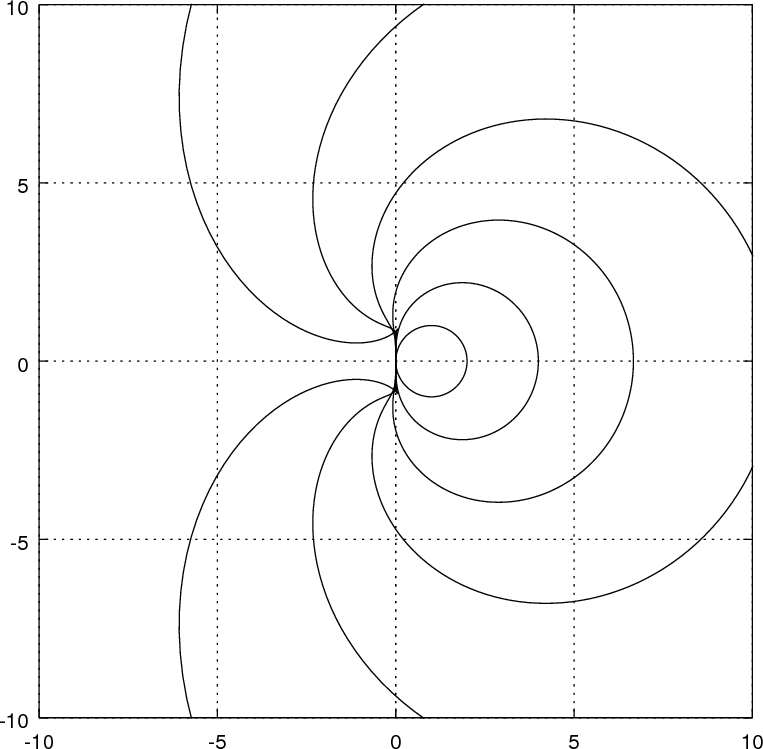
\includegraphics[width=.45\textwidth]{fig/stability-bdf.png}
  \hfill
  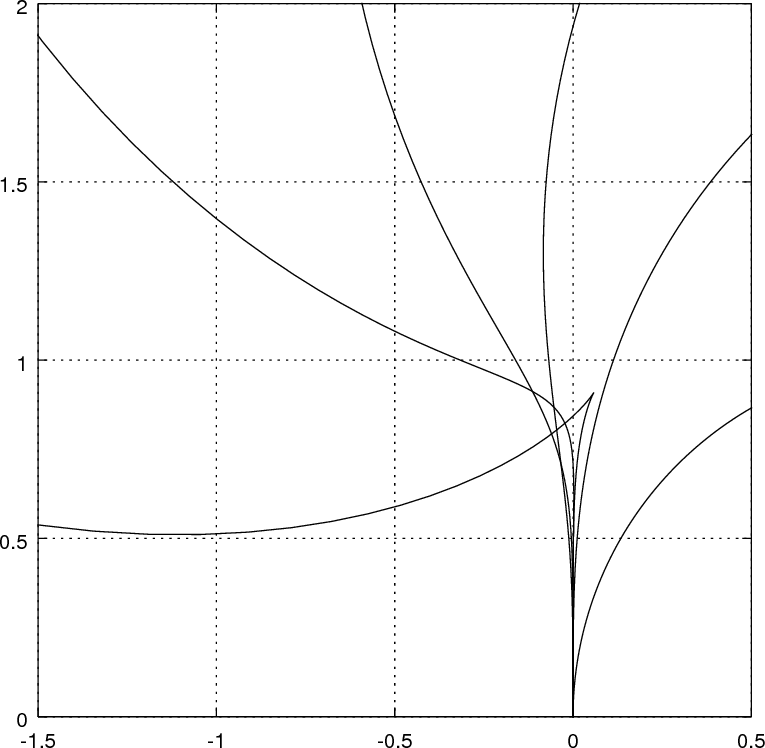
\includegraphics[width=.45\textwidth]{fig/stability-bdf-zoom.png}
  \caption{Boundaries of stability regions of BDF1 to BDF6. Unstable
    region right of the origin. Zoom on the right}
  \label{fig:bdf-stability}
\end{figure}
\begin{table}[tp]
  \centering
  \begin{tabular}{c|cccccc}
    $k$ & 1 & 2 & 3 & 4 & 5 & 6 \\\hline
    $\alpha$ & 90$^\circ$ & 90$^\circ$& 86.03$^\circ$
                    & 73.35$^\circ$& 51.84$^\circ$
                            & 17.84$^\circ$ \\
    $D$ & 0 & 0 & 0.083& 0.667& 2.327& 6.075
  \end{tabular}
  \caption{Values for A($\alpha$)- and stiff stability for BDF methods
    of order $k$.}
  \label{tab:bdf-stability}
\end{table}

%%%%%%%%%%%%%%%%%%%%%%%%%%%%%%%%%%%%%%%%%%%%%%%%%%%%%%%%%%%%%%%%%%%%%%
\section{Predictor-corrector schemes}

\begin{Definition*}{predictor-corrector}{Predictor-corrector methods}
  Assume a pair of time stepping schemes, one explicit, one implicit,
  \begin{align*}
    \hat y_{k} &= \hat \verfahren_p(y_{k-1}) \\
    y_k &= \verfahren_c(y_{k-1},y_{k}),
  \end{align*}
  we can use $\hat y_k$ as initial value for the Newton iteration for
  $y_k$. In an extreme case, we let
  \begin{gather*}
    y_k = \verfahren_c(y_{k-1},\hat y_{k}),
  \end{gather*}
  without any further iteration.
\end{Definition*}

\begin{remark}
  Predictor-corrector methods were developed strongly around
  Adams-Moulton and Adams-Bashforth methods, since the implicit ones
  have much smaller error constants. Given that these methods offer no
  considerable advantages compared to Runge-Kutta methods, but
  stability properties and implementation are weak points, We omit
  their discussion.

  A simple predictor for BDF methods can be obtained, since they are
  based on an interpolating polynomial. Thus, we simply extrapolate
  this polynomial to the next point in time.
\end{remark}

\begin{example}
  While the predictor-corrector idea sounds reasonable, we have to be
  careful with stiff problems, the original reason for using implicit
  methods. Take again our favorite IVP
  \begin{gather*}
    u' = \lambda u,
    \qquad u(0) = 1.
  \end{gather*}
  We apply the BDF(1) scheme, namely the implicit Euler method, with
  step size 1. According to its stability
  function~\eqref{eq:impl:stabil:impleuler}, we obtain
  \begin{gather*}
    y_1 = \frac1{1-\lambda}.
  \end{gather*}
  Hence, the interpolating polynomial is
  \begin{gather*}
    y(t) = (1-t) + \frac1{1-\lambda} t = 1 + \frac{\lambda}{1-\lambda}t.
  \end{gather*}
  For the mildly stiff problem $\lambda = -3$, we obtain
  \begin{gather*}
    y_1 = 0.25, \qquad y_2 = 0.0625,
    \qquad \hat y_2 = y(2) = -0.5.
  \end{gather*}
  Thus, the extrapolated value is already a much worse initial value
  for a Newton iteration than using the value from the previous time
  step.
  
  While this example was particularly chosen to exhibit such failure,
  it does show that extrapolation of stiff problems has its
  pitfalls. Here, we end up with a time step restriction which is
  comparable to the stability condition of the explicit method.
\end{example}


%%% Local Variables: 
%%% mode: latex
%%% TeX-master: "notes"
%%% End: 


\begin{remark}
  \index{step size!constant} The LMM was defined for constant step size
  $h$.  In principle it is possible to implement the method with a
  variable step size but we restrict ourselves to the constant case.
  Notes to the step size control can be found later on in this chapter.
\end{remark}

\begin{remark}
  One-step methods were always denoted by describing how to compute
  $y_1$ from $y_0$. Here, the notation becomes more complicated, but
  sometimes we consider only $y_s$ computed from $y_0,\dots,y_{s-1}$
  implying the same rues for $y_k$ computed from
  $y_{k-\lmms},\dots,y_{k-1}$.
\end{remark}
\begin{Definition}{lmm-errors}
    \index{Lh@$L_h$|textbf}
  We express the LMM with the linear \define{difference operator}
  \begin{gather}
    \label{eq:lmm:9}
    (L_hu)(t_k) = \sum_{r=0}^{\lmms}\Bigl(\alpha_{\lmms-r} u(t_{k-r}) - h
    \beta_{R-r} f\bigl(t_{k-r},u(t_{k-r})\bigr)\Bigr)
  \end{gather}
  and for a continuous function $u$ we define the \textbf{truncation
    error}\defindex{truncation error!LMM}
  \begin{gather}
    \label{eq:lmm:10}
    \tau_h(t_k) = \tfrac1hL_hu(t_k).
  \end{gather}
  The \textbf{local error} \defindex{LMM!local error}\defindex{local
    error!LMM} of a linear multistep method is defined by
  \begin{gather*}
    u(t_\lmms) - y_\lmms
  \end{gather*}
  where $u(t)$ denotes the exact solution of $u' = f(t,u), u(t_0)=u_0$
  and $y_s$ the numerical solution by using the exact initial values
 	$y_i = u(t_i)$ for $i = 0,1,...,s-1$.
\end{Definition}

%%% Local Variables:
%%% mode: latex
%%% TeX-master: "../notes"
%%% End:


\begin{lemma}
  Consider the differential equation
  \begin{gather*}
    y' = f(t,y) \qquad y(t_0) = y_0
  \end{gather*}
  where f is given continuously differentiable and $y(t)$ is the exact solution.
  For the local error we obtain

  \begin{gather}
    y(t_k)-y_k = \left( \alpha_0 \identity - h\beta_0 \frac{\partial f}{\partial y}(t_k,\eta) \right)^{-1} (L_h u)(t_k).
  \end{gather}

  Here $\eta$ is a value between $y(t_k)$ and $y_k$ if $f$ is a scalar
	function.
  If $f$ is multidimensional, the matrix 
	$\frac{\partial f}{\partial y}(t_k,\eta)$ is the Jacobi matrix, 
	which rows are evaluated at possible places between
	$y(t_k)$ and $y_k$.
\end{lemma}

\begin{proof}
  Considering the local error we can assume exact initial values 
  and therefore we can transform ~\ref{eq:lmm:4} to:
  \begin{gather*}
    \alpha_\lmms y_k + \sum\limits_{r=1}^\lmms \alpha_{\lmms-r} y(t_{k-r})
    = h \left( \beta_\lmms f_k + \sum\limits_{r=1}^\lmms \beta_{\lmms-r} f_{k-r} \right)
  \end{gather*}
  We transform further:
  \begin{multline*}
    \sum\limits_{r=0}^{\lmms} \left( \alpha_r y(t_{k-r})
      - h \beta_r f(t_{k-r},y(t_{k-r})) \right)
    \\
    - \alpha_0 y(t_k) + h \beta_0 f(t_k, y(t_k)) + \alpha_0 y_k
    - h \beta_0 f(t_k,y_k) = 0.
  \end{multline*}
	We now insert ~\ref{eq:lmm:9} which results in
  \begin{gather*}
    (L_h u)(t_k) = \alpha_0 \left( y(t_k) - y_k \right) - h \beta_0 \left( f(t_k,y(t_k)) - f(t_k,y_k) \right)
    \\
    \left( y(t_k) - y_k \right) \left( \alpha_0 \identity - h \beta_0 \frac{f(t_k,y(t_k)) - f(t_k,y_k)}{y(t_k) - y_k} \right)
  \end{gather*}
  By application of the mean value theorem and 
  subsequent transformation we obtain the statement of the theorem.
\end{proof}

      % \cite[Lemma 2.2, p. 369]{HairerNorsettWanner93}

\begin{Definition}{lmm-consistency}
  An LMM is consistent of order $p$, if for all sufficient regular
  functions $u$ and all relevant $k$ there holds
  \begin{gather}
    \label{eq:lmm:11}
    \tau_h(t_k) = \mathcal O(h^p),
  \end{gather}
  or equivalently, that the \putindex{local error} is $\mathcal O(h^{p+1})$.
\end{Definition}

%%% Local Variables:
%%% mode: latex
%%% TeX-master: "../notes"
%%% End:

\begin{Lemma}{lmm-bramble-hilbert}
  An LMM is consistent of order $p$ if and only if for all polynomials
  $\phi_q$ of degree $q \le p$ and $f(t,q(t)) = q'(t)$ there holds:
  \begin{gather}
    \label{eq:lmm:14}
    L_h \phi_q = 0.
  \end{gather}
\end{Lemma}

%%% Local Variables:
%%% mode: latex
%%% TeX-master: "../notes"
%%% End:


\begin{proof}
  We start with the Taylor expansion of a solution $u$ of the ODE and
  the corresponding right hand side $f$ for $t_k$, where we insert,
  unlike usual, $f=u'$:
  \begin{alignat*}2
    u(t) &= \sum_{i=0}^p \frac{u^{(i)}(t_k)}{i!}(t-t_k)^i +
    \frac{u^{(p+1)}(\xi)}{(p+1)!}(t-t_k)^{p+1} &=:& \phi(t) + r_u(t)
    \\
    f\bigl(t,u(t)\bigr) &= \sum_{i=1}^p \frac{u^{(i)}(t_k)}{(i-1)!}(t-t_k)^{i-1} +
    \frac{u^{(p+1)}(\xi)}{p!}(t-t_k)^{p} &=:& \phi'(t) + r_f(t),
  \end{alignat*}
  with the Taylor polynomial $\phi(t)$ of degree $p$ and remainder
  $r_u(t)$ and $r_f(t)$. Out of this we calculate:
  \begin{align*}
    L_h u(t_k) =& \sum_{r=0}^\lmms \alpha_{\lmms-r} \phi(t_{k-r}) - h
    \sum_{r=0}^\lmms \beta_{\lmms-r} \phi'(t_{k-r})
    \\
    &+ \sum_{r=0}^\lmms \alpha_{\lmms-r} r_u(t_{k-r}) - h
    \sum_{r=0}^\lmms \beta_{\lmms-r} r_f(t_{k-r}).
  \end{align*}
  Since $t_{k-r}-t_k = r h$, the first row equals a polynomial 
  $\psi(h)$ in $h$ of degree $p$. For the second row we insert the
	reminder estimate $r_u(t) = \mathcal O((t-t_k)^{p+1}) = h
  r_f(t)$ and get:
  \begin{gather}
    \label{eq:lmm:15}
    L_h u(t_k) = L_h \phi(t_k) + \mathcal O(h^{p+1}) = \psi(h) + \mathcal O(h^{p+1}).
  \end{gather}
  According to the definition of the truncation error, this term has to be of
	order $p+1$, such that the method is of order $p$. However it is $\psi$
  of degree $p$. This can only hold true if $L_h\phi=\psi\equiv
  0$. On the other hand $\tau_h(t_k)$ automatically is of order
  $p$. Since $u$ is the solution of an arbitrary right hand side, this
	condition has to be satisfied for all kind of Taylor polynomials $\phi$ 
	of degree $p$.
\end{proof}

\begin{Theorem}{lmm-consistency}
  \index{step size!constant}
  A LMM with constant step size is consistent of order
  $p$ if and only if
    \begin{gather}
      \label{eq:lmm:12}
      \begin{split}
      \sum_{r=0}^\lmms \alpha_{r} &= 0, \\
      \sum_{r=0}^\lmms \bigl(\alpha_{r}r^q - q \beta_{r}
      r^{q-1}\bigr) &= 0,
      \qquad q = 1,\dots,p        
      \end{split}
    \end{gather}
\end{Theorem}


\begin{proof}
  According to lemma~\ref{Lemma:lmm-bramble-hilbert} it is sufficient
  to show that ~\eqref{eq:lmm:12} is equivalent to $L_h \phi_q=0$ for
  polynomials of degree $q\le p$. Due to linearity of the method it
  however is sufficient to show this for a basis of the polynomial
  space of degree $p$.  For that we choose the monomial basis of the
  form
  \begin{gather*}
  \pi_q(t) =
  \left(\frac{t-t_{k-\lmms}}h\right)^q,\qquad q=0,\dots,p.
  \end{gather*}
  For those it holds: $\pi_q(t_{k-r}) = (\lmms-r)^q$. Now we see that
  the first condition is $L_h\pi_0 = 0$ (here is
  $\pi_0'\equiv0$) and the second condition is $L_h\pi_q = 0$.
\end{proof}

\begin{todo}
  Beispiel einer konsistenten LMM, die nicht konvergiert.
\end{todo}

\begin{remark}
  As shown in a homework problem, a consistent LMM is not necessary
  convergent. To understand this behavior and develop criteria for
  convergence we need to diverge into the theory of difference
  equations.
\end{remark}
%%%%%%%%%%%%%%%%%%%%%%%%%%%%%%%%%%%%%%%%%%%%%%%%%%%%%%%%%%%%%%%%%%%%%%
%%%%%%%%%%%%%%%%%%%%%%%%%%%%%%%%%%%%%%%%%%%%%%%%%%%%%%%%%%%%%%%%%%%%%%
\section{Properties of difference equations}
%%%%%%%%%%%%%%%%%%%%%%%%%%%%%%%%%%%%%%%%%%%%%%%%%%%%%%%%%%%%%%%%%%%%%%
%%%%%%%%%%%%%%%%%%%%%%%%%%%%%%%%%%%%%%%%%%%%%%%%%%%%%%%%%%%%%%%%%%%%%%

\begin{intro}
  The stability of LMM can be understood by employing the fairly old
  theory of difference equations. In order to keep the presentation
  simple in this section, we use a different notation for numbering
  indices in the equations. Nevertheless, the coefficients of the
  characteristic polynomial are the same as for LMM.
\end{intro}

\begin{Definition}{difference-equation}
  An equation of the form
  \begin{gather}
    \label{eq:lmm:3}
    \sum_{r=0}^\lmms \alpha_{r} y_{n+r} = 0
  \end{gather}
  is called a homogeneous \define{difference equation}. A sequence
  $\{y_n\}_{n=0,\dots,\infty}$ is solution of the difference equation,
  if the equation holds true for all $n\ge \lmms$. The values
  $y_n$ may be from any of the spaces $\R$, $\C$, $\R^d$ or $\C^d$.

  The \define{generating polynomial} of this difference equation
  is
  \begin{gather}
    \label{eq:lmm:2}
    \chi(x) = \sum_{r=0}^\lmms \alpha_{r} x^{r}.
  \end{gather}

\end{Definition}

%%% Local Variables:
%%% mode: latex
%%% TeX-master: "../notes"
%%% End:


\begin{Lemma}{lmm:1}
  The solutions of the equation~\eqref{eq:lmm:3} with $y_n\in \R$ or
  $y_n\in \C$ form a vector space of dimension $\lmms$. 
\end{Lemma}

\begin{proof}
  Since the equation~\eqref{eq:lmm:3} is linear and homogeneous, it is
  obvious that if two sequences of solutions $\{y^{(1)}\}$ and
  $\{y^{(2)}\}$ satisfy the equation, sums of multiples of them
  satisfy it too.

  As soon as the initial values $y_0$ to $y_{\lmms-1}$ are chosen, all
  other sequence members are uniquely defined.  Moreover it holds
  \begin{gather*}
    y_0=y_1=\dots=y_{\lmms-1}=0
    \quad\Longrightarrow\quad
    y_n = 0, \;n \ge 0.
  \end{gather*}
  Therefore it is sufficient to consider the first $\lmms$ values.  If
  they are linear independent, then the overall sequences are and vice
  versa. Thus, the initial values form a $\lmms$
  dimensional vector space.
\end{proof}

\begin{Lemma}{difference-equation-solutions}
  For each root $\xi$ of the generating polynomial $\chi(x)$ the
  sequence $y_n = \xi^n$ is a solution of the difference
  equation~\eqref{eq:lmm:3}.
\end{Lemma}


%%% Local Variables: 
%%% mode: latex
%%% TeX-master: "../notes"
%%% End: 


\begin{proof}
  Inserting of the solution $y_n = \xi^n$ into the difference equation
  results in
  \begin{gather*}
    \sum_{r=0}^\lmms \alpha_{r} \xi^{n+r} = \xi^{n}
    \sum_{r=0}^\lmms \alpha_{r} \xi^{r}
    = \xi^{n} \chi(\xi) = 0.
  \end{gather*}
\end{proof}

\begin{Theorem}{difference-equation-basis}
  Let $\{\xi_i\}_{i=1,\dots,\iota}$ be the roots of the
  generating polynomial $\chi$ with multiplicity $\nu_i$. Then,
  the sequences of the form
  \begin{gather}
    \label{eq:lmm:6}
%    y^{(i,k)}_n = p_k(n)\xi_i^n
    y^{(i,k)}_n = n^{k-1}\xi_i^n
    \quad i=1,\dots,\iota; \quad k = 1,\dots,\nu_i
  \end{gather}
%  mit den Polynomen
%  \begin{gather*}
%    p_0(n) = 1 \quad p_k(n) = \prod_{\kappa=0}^{k-1} (n-\kappa)
%  \end{gather*}
  form a basis of the solution space of the difference
  equation~\eqref{eq:lmm:3}.
\end{Theorem}


%%% Local Variables: 
%%% mode: latex
%%% TeX-master: "../notes"
%%% End: 


\begin{proof}
  First we observe that the sum of the multiplicities of the roots
  results in the degree of the polynomial:
  \begin{gather*}
    \lmms = \sum_{i=1}^\iota \nu_i.
  \end{gather*}
  Moreover we know because of Lemma~\ref{Lemma:lmm:1}, that $\lmms$ is
  the dimension of the solution space. We show that the sequences
  $\{y^{(i,k)}_n\}$ are linear independent. This is clear for
  sequences of different index $i$. It is also clear for different roots,
  because for $n\to\infty$ the exponential function nullifies the
  influence of the polynomials.
  
  It remains to show that the sequences $\{y^{(i,k)}_n\}$ in fact are
  solutions of the difference equations.  For $k=0$ we have proven
  this already in lemma~\ref{Lemma:difference-equation-solutions}.  We proof the fact here for
  $k=2$ and for a double zero $\xi_i$; the principle for higher order
  roots should be clear then.  Equation~\eqref{eq:lmm:3} applied to
  the sequence $\{n \xi_i^n\}$ results in
  \begin{align*}
    \sum_{r=0}^{\lmms} \alpha_r (n+r) \xi_i^{n+r}
    &= n \xi_i^n \sum_{r=0}^{\lmms} \alpha_r \xi_i^{r}
    + \xi_i^{n+1} \sum_{r=1}^{\lmms} \alpha_r r \xi_i^{r-1}
    \\
    &= n \xi_i^n \rho(\xi_i) + \xi_i^{n+1} \rho'(\xi_i) = 0.
  \end{align*}
  Here the term with $\alpha_0$ vanishes, because it is multiplied
  with $r=0$. $\rho(\xi_i) = \rho'(\xi_i) = 0$ because $\xi_i$ is a
  multiple root.
\end{proof}

\begin{Corollary*}{root-test}{Root test}
  All solutions $\{y_n\}$ of the difference equation~\eqref{eq:lmm:3}
  are bounded for $n\to\infty$ if and only if it holds:
  \begin{itemize}
  \item all roots of the generating polynomial $\chi(x)$
    lie in the closed unit circle $\bigl\{z\in \C \big|\; |z|\le
    1\bigr\}$ and
  \item all roots on the boundary of the unit circle are simple.
  \end{itemize}
\end{Corollary*}

%%% Local Variables: 
%%% mode: latex
%%% TeX-master: "../notes"
%%% End: 


\begin{proof}
  According to theorem~\ref{Theorem:difference-equation-basis} we can write all solutions
  as linear combinations of the sequences $y^{(i,k)}$ in
  equation~\eqref{eq:lmm:6}. Therefore,
  \begin{enumerate}
  \item all solutions to $|\xi_i|<1$ for $n\to\infty$ converge to zero
  \item all solutions to $|\xi_i|>1$ for $n\to\infty$ converge to infinity
  \item all solutions to $|\xi_i|=1$ for $n\to\infty$ stay bounded 
	if and only if $\xi_i$ is simple.
  \end{enumerate}
  This proves the statement of the theorem.
\end{proof}

%%%%%%%%%%%%%%%%%%%%%%%%%%%%%%%%%%%%%%%%%%%%%%%%%%%%%%%%%%%%%%%%%%%%%%
%%%%%%%%%%%%%%%%%%%%%%%%%%%%%%%%%%%%%%%%%%%%%%%%%%%%%%%%%%%%%%%%%%%%%%
\section{Stability and convergence}
%%%%%%%%%%%%%%%%%%%%%%%%%%%%%%%%%%%%%%%%%%%%%%%%%%%%%%%%%%%%%%%%%%%%%%
%%%%%%%%%%%%%%%%%%%%%%%%%%%%%%%%%%%%%%%%%%%%%%%%%%%%%%%%%%%%%%%%%%%%%%

\begin{remark}
  In contrast to one-step methods the convergence of multistep methods
  follows not directly from the consistency of the method, if the
  right hand side of the differential equation satisfies the Lipschitz
  condition~\eqref{eq:awa:1}.  Analog to the A-stability we will
  discuss this by means of a simple model problem and we will deduce
  stability conditions.
\end{remark}

\begin{remark}
  In the following we investigate the solution to a fixed point in time
  $t$ with a shrinking step size $h$. Therefore we choose $n$
  steps of step size $h = t/n$ and let $n$ go towards infinity.
\end{remark}

\begin{Theorem}{lmm-stability}
  A LMM is stable if and only if all roots of the first
  generating polynomial $\rho(x)$ of equation~\eqref{eq:lmm:5} lie
  in the unit circle of the complex plane and all roots on the
  boundary of the unit circle are simple.
\end{Theorem}


%%% Local Variables: 
%%% mode: latex
%%% TeX-master: "../notes"
%%% End: 

\begin{Theorem}{lmm-stability}
  A LMM is stable if and only if all roots of the first
  generating polynomial $\rho(x)$ of equation~\eqref{eq:lmm:5} lie
  in the unit circle of the complex plane and all roots on the
  boundary of the unit circle are simple.
\end{Theorem}


%%% Local Variables: 
%%% mode: latex
%%% TeX-master: "../notes"
%%% End: 


\begin{proof}
  The application of the LMM to the equation~\eqref{eq:lmm:1} results
  in the difference equation
  \begin{gather*}
    \sum_{r=0}^{\lmms} \alpha_{\lmms-r} y_{n-r} = 0.
  \end{gather*}
  Now we have to proof that the solutions for fixed $t = h n$ stay
  bounded if $h\to 0$. But we also see that the upper equation does
  not contain $h$. Therefore we have to examine, if the solutions
  $y_n$ stay bounded for $n\to \infty$.  By resorting the summation we
  obtain a difference equation of the form~\eqref{eq:lmm:3}. Due to
  corollary~\ref{Corollary:root-test} it follows the statement of the theorem.
\end{proof}

\begin{Corollary}{adams-stability}
  Adams-Bashforth and Adams-Moulton methods are stable.
\end{Corollary}

\begin{proof}
  For all of these methods the first generating polynomial is $\rho(x)
  = x^\lmms-x^{\lmms-1}$. It has the simple root $\xi_1 = 1$ and the
  $\lmms-1$-fold root 0.
\end{proof}

\begin{Theorem}{BDF-stability}
  The BDF methods are stable for $\lmms \le 6$ and not
  stable for $\lmms \ge 7$.
\end{Theorem}

\begin{Theorem}{lmm-convergence}
  If a linear multi-step method is stable and consistent of order $p$,
  then it is convergent of order $p$.
\end{Theorem}

%%% Local Variables: 
%%% mode: latex
%%% TeX-master: "../notes"
%%% End: 

\begin{Lemma}{lmm-one-step}
  Every multistep method can be recast as a one-step method
  \begin{gather}
    \label{eq:lmm-one-step:1}
    Y_{k} = (A \otimes \identity) Y_{k-1} + h \verfahren_h(t_{k-1}, Y_{k-1})
  \end{gather}
  where with $\alpha_r' = \alpha_r/\alpha_s$
  \begin{gather}
    \label{eq:lmm-one-step:2}
    Y_k =
    \begin{pmatrix}
      y_k \\ \vdots \\ y_{k-s+1}
    \end{pmatrix},
    \quad
    A =
    \begin{pmatrix}
      -\alpha_{\lmms-1}' & -\alpha_{\lmms-2}' & \cdots & -\alpha_{0}'\\
      1 & 0 & \cdots & 0 \\
      & \ddots & \cdots & 0 \\
      & & 1 & 0
    \end{pmatrix},
  \end{gather}
  and $\verfahren_h(t_k, Y_k) = (e_1 \otimes \identity) \psi_h(t_{k-1}, Y_{k-1})$ with
  $\beta_r' = \beta_r/\alpha_s$ and $\psi_h$ defined implicitly by
  \begin{multline}
    \label{eq:lmm-one-step:3}
    \psi_h(t_{k-1}, Y_{k-1})
    =\sum_{r=1}^{\lmms} \beta_{\lmms-r} f(t_{k-r},y_{k-r})
    \\
    + \beta_s' f\left(t_k, h\psi_h(t_{k-1}, Y_{k-1}) -
      \sum_{r=1}^{\lmms} \alpha_{\lmms-r}' y_{k-r}\right).
  \end{multline}
\end{Lemma}

%%% Local Variables: 
%%% mode: latex
%%% TeX-master: "../notes"
%%% End: 


\begin{proof}
  From the general form of LMM we
  obtain
  \begin{gather*}
    \frac1{\alpha_s} \sum_{r=0}^\lmms \alpha_{\lmms-r} y_{k-r}
    = \frac{h}{\alpha_s} \sum_{r=0}^{\lmms-1} \beta_{\lmms-r} f_{k-r}
    + \beta_s f_k.
  \end{gather*}
  We rewrite this to
  \begin{gather*}
    y_k = -\sum_{r=1}^{\lmms} \alpha'_{\lmms-r} y_{k-r} +
    h\psi_h(t_{k-1}, Y_{k-1}),
  \end{gather*}
  where we implicitly enter this formula as value for $y_k$ in the
  computation of $f_k$. It remains to realize that this is the first
  set of $d$ equations in~\eqref{eq:lmm-one-step:1}, and that the
  remaining ones are just shifting $y_i$ to $y_{i+1}$.
\end{proof}

\begin{Lemma}{lmm-one-consistency}
  Let $u(t)$ be the exact solution of the IVP. For $k=s,\ldots$, we
  define the vector $\widehat Y_{k}$ as the solution of a single step
  \begin{gather*}
    \widehat Y_{k} = (A\otimes I) U_{k-1} + h \verfahren_h(t_{k-1} U_{k-1}),
  \end{gather*}
  with correct initial values $U_{k-1} =
  (u_{k-1},u_{k-2},\dots,u_{k-\lmms})^T$.
  
  If the multistep method is consistent of order $p$, and $f$ is
  sufficiently smooth, then there exist constants $h_0>0$  and $M$
  such that for $h\le h_0$ there holds
  \begin{gather}
    \label{eq:lmm-one-consistency:1}
    \norm{Y_k-\widehat Y_h} \le M h^{p+1}.
  \end{gather}
\end{Lemma}

%%% Local Variables: 
%%% mode: latex
%%% TeX-master: "../notes"
%%% End: 


\begin{proof}
  The first component of $Y_k - \widehat Y_k$ is the local error of
  step $k$, which is of order $h^{p+1}$ by the assumption. The other
  components vanish by the definition of the method.
\end{proof}

\begin{Lemma}{lmm-one-stability}
  Assume that an LMM is stable. Then, there exists a vector norm on
  $\C^{\lmms d}$ such that the operator norm of the matrix $A$
  satisfies
  \begin{gather}
    \label{eq:lmm-one-stability:1}
    \norm{A\otimes \identity} \le 1.
  \end{gather}
\end{Lemma}

%%% Local Variables: 
%%% mode: latex
%%% TeX-master: "../notes"
%%% End: 


\begin{proof}
  We notice that $\widehat\rho(x) = \sum \alpha'_{s-r} x^r$ is the
  characteristic polynomial of the matrix $A$ and thus its eigenvalues
  are the roots of $\widehat\rho(x)$, which has the same roots as the
  generating polynomial $\rho(x)$. By the root test, we know that
  simple roots, which correspond to irreducible blocks of dimension
  one have maximal modulus one. Furthermore, every Jordan block of
  dimension greater than one corresponds to a multiple root, which by
  assumption has modulus strictly less than one. It is easy to see
  that such a block admits a modified canonical form
  \begin{gather*}
    J_i =
    \begin{pmatrix}
      \lambda_i & 1- \abs{\lambda_i}\\
        & \lambda_i &\ddots\\
          &&\ddots & 1- \abs{\lambda_i}\\
            &&&\lambda_i
    \end{pmatrix}.
  \end{gather*}
  Thus, the canonical form $J = T^{-1}AT$ has norm $\norm{J}_{\infty}
  \le 1$. If we define the norm
  \begin{gather*}
    \norm{x} = \norm{(T^{-1}\otimes I)x}_\infty,
  \end{gather*}
  we obtain the result by
  \begin{multline*}
    \norm{(A\otimes I)x}
    = \norm{(T^{-1}\otimes I)(A\otimes I)x}_\infty
    = \norm{(J\otimes I)(T^{-1}\otimes I)x}_\infty
    \\
    \le \norm{(T^{-1}\otimes I)x}_\infty
    = \norm{x}.
  \end{multline*}
\end{proof}

\begin{Theorem}{lmm-convergence}
  If a linear multi-step method is stable and consistent of order $p$,
  then it is convergent of order $p$.
\end{Theorem}

%%% Local Variables: 
%%% mode: latex
%%% TeX-master: "../notes"
%%% End: 


\begin{proof}
  We reduce the proof to convergence of a one-step method with
  \begin{gather}
    \label{eq:lmm:18}
    Y_k = G(Y_{k-1}) =  (A\otimes I) Y_{k-1} + h \verfahren_h(t_{k-1}, Y_{k-1}).
  \end{gather}
  Let $Y_{k-1}$ and $Z_{k-1}$ be two initial values for the interval $I_k$.
  By the previous lemma, we have in the norm defined there, for
  sufficiently small $h$, and assuming a Lipschitz constant $L_h$ for
  $\verfahren_h$ :
  \begin{gather}
    \label{eq:lmm:19}
    \norm{G(Y_{k-1})-G(Z_{k-1})} \le (1+h L_h) \norm{Y_{k-1}-Z_{k-1}}.
  \end{gather}
  Thus, the local error $\eta_k = U_k - \widehat Y_k$ at step $k$, which by
  Lemma~\ref{Lemma:lmm-one-consistency} is bounded by $M h^{p+1}$, accumulates
  until step $n$ at most to $h^{p+1}(1_h L_h)^{n-k}$.

  We have:
  \begin{align*}
    \norm{U_1 - Y_1} &\le (1+h L_h)\norm{U_0-y_0} + M h^{p+1} \\
    \norm{U_2 - Y_2} &\le (1+h L_h)^2\norm{U_0-y_0} +  M h^{p+1} \bigl(1+ (1+h L_h)\bigr)\\
    \norm{U_3 - Y_3} &\le (1+h L_h)^3\norm{U_0-y_0} +  M h^{p+1} \Bigl(\bigl(1+ (1+h L_h)+ (1+h L_h)^2\bigr)\Bigr)\\
    \norm{U_n-Y_n} &\le e^{n h L_h}\norm{U_0-Y_0} +
    \frac{M h^p}{L_h}\bigl(e^{n h L_h} - 1\bigr).
  \end{align*}
\end{proof}

\subsection{Starting procedures}

\begin{intro}
In contrast to one-step methods, where the numerical solution is obtained 
solely from the differential equation and the initial value, multistep 
methods require more than one start value. An LMM with $s$ steps requires $s$ 
known start values $y_{k-s}, \dots, y_{k-1}$. Mostly, they are not provided 
by the IVP itself. Thus, general LMM decompose into two parts: 
\begin{itemize}
\item a \emph{starting phase} where the start values are computed in a 
suitable way and
\item a \emph{run phase} where the LMM is executed. 
\end{itemize}
It is crucial that the method of the starting phase provides a suitable order 
corresponding to the LMM of the run phase, recall Definition 
\ref{Definition:lmm-convergence}. Moreover, it should have analog properties to 
the LMM, like explicit/implicit or applicability to stiff problems. 
% We now consider different starting procedures for an implicit LMM with 
% convergence order $p$. According to Definition \ref{Definition:lmm-convergence} 
% the starting values are required to have the same convergence order. 
Possible choices for the starting phase include multistep methods with variable 
order and one-step methods.  
\end{intro}

\begin{example}[Self starter]
A 2-step BDF method requires $y_0$ and $y_1$ to be known. $y_0$ is given by the 
initial value while $y_1$ is unknown so far. To guarantee that the method has 
order 2, $y_1$ needs to be locally of order 2 at least
\begin{align}\label{eq:lmm_1BDFstarter}
|u(t_1)-y_1| \leq c_0 h^2.
\end{align}
This is ensured, for example, by one step of the 1-step BDF method.

However, starting an LMM with $s>2$ steps by a first-order method and then 
successively increasing the order until $s$ is reached does not provide the 
desired global order. That is due to the fact that the first step limits  
the overall convergence order to 2, compare \eqref{eq:lmm_1BDFstarter}. 
Nevertheless, self starters are often used in practice. 
\end{example}
% In this case local 
% error estimates are used to bound the errors of the starting values and all 
% approximations of the run phase by reducing the step sizes, 
% %. Moreover, also in 
% %the run phase the step sizes are controlled using local error estimates, 
% see the  
% discussion on step size control in Section \ref{section:step_size_control}. 


\begin{example}[Runge-Kutta starter]
\label{Example:RKstarter}
One can use Runge-Kutta methods to start LMM. Since only a fixed
number of starting steps are performed, the local order of the
Runge-Kutta approximation is crucial.  For an implicit LMM with
convergence order $p$ and stepsize $h$ one could use an RK method with
consistency order $p-1$ with the same stepsize $h$.

Consider a 3-step BDF method. Thus, beside $y_0$, we need start values 
$y_1, y_2$ with errors less than $c_0 h^3$. They can be computed by RK methods 
of consistency order $2$, for example by two steps of the 1-stage Gau\ss \ 
collocation method with step size $h$ since it has consistency order $2s=2$, 
see theorem \ref{Theorem:gauss-consistency}.
\end{example}




\begin{example}[Continuous Runge-Kutta starter]
  Another option is to use continuous Runge-Kutta methods and to
  evaluate the continuous approximation to obtain the required
  starting values.

  In constrast to Example \ref{Example:RKstarter} one could also use
  the continuous polynomial approximation of Gau\ss \ collocation to
  start a 3-step BDF method. One step with step size $2h$ of a 2-stage
  Gau\ss \ collocation method would give a polynomial of degree $2$
  which is then evaluated in $t_1=t_0+h$ and $t_2=t_1+h$ to obtain
  $y_1, y_2$. According to Theorem
  \ref{Theorem:collocation-continuous} $y_1, y_2$ have the appropriate
  order.
\end{example}

\begin{remark}
  In practice not the order of a procedure is crucial but rather the
  fact that the errors of all approximations (the start values and all
  approximations of the run phase) are bounded by the user-given
  tolerance, compare Section \ref{section:step_size_control}. Thus,
  the step sizes of all steps are controlled using local error
  estimates. Hence, self starting procedures usually start with very
  small step sizes and increase them successively. Due to their higher
  orders RK starters usually are allowed to use moderate step sizes in
  the beginning. Generally, LMM are applied with variable step sizes
  and orders in practice (see e.g. Exercise 7.2).
\end{remark}



%%%%%%%%%%%%%%%%%%%%%%%%%%%%%%%%%%%%%%%%%%%%%%%%%%%%%%%%%%%%%%%%%%%%%%
%%%%%%%%%%%%%%%%%%%%%%%%%%%%%%%%%%%%%%%%%%%%%%%%%%%%%%%%%%%%%%%%%%%%%%
\section{LMM and stiff problems}
%%%%%%%%%%%%%%%%%%%%%%%%%%%%%%%%%%%%%%%%%%%%%%%%%%%%%%%%%%%%%%%%%%%%%%
%%%%%%%%%%%%%%%%%%%%%%%%%%%%%%%%%%%%%%%%%%%%%%%%%%%%%%%%%%%%%%%%%%%%%%

\begin{Definition*}{lmm-stability-region}{A-stability of LMM}
  \index{stability region!of a LMM}
  The linear model difference equation
  \begin{gather}
    \label{eq:lmm:7}
    \sum_{r=0}^{\lmms} \bigl(\alpha_{\lmms-r} - z \beta_{\lmms-r}) y_{n-r}.
  \end{gather}
  is obtained by applying an LMM to the model equation
  $u' = \lambda u$ and inserting $z=h\lambda$.

  The \define{stability region} of an LMM is the set of points $z\in \C$,
  for which all solution sequences $\{y_n\}$ of the equation~\eqref{eq:lmm:7}
  stay bounded for $n\to\infty$. An LMM is called \define{A-stable}, if the 
  stability region contains the left half-plane of $\C$.
\end{Definition*}


\begin{Definition}{lmm-stability-polynomial}
  The stability polynomial of an LMM is obtained by inserting
  $y_n = x^n$ into the linear model difference equation to obtain
  \begin{gather}
    \label{eq:lmm:8}
    r_z(x) = \sum_{r=0}^{\lmms} \bigl(\alpha_{\lmms-r} - z \beta_{\lmms-r})
    x^{\lmms-r}.
  \end{gather}
\end{Definition}

\begin{remark}
  Instead of the simple amplification function $r(z)$ of the one-step
  methods, we get here a function of two variables.  The point $z$ for
  which we want to show stability and the artificial variable $x$ from
  the analysis of the method.
\end{remark}

\begin{Lemma}{lmm-stability}
  Let $\{\xi_1(z),\dots,\xi_\lmms(z)\}$ be the set of roots of the
  stability polynomial $r_z(x)$ as functions of $z$.
  A point $z\in \C$ is in the stability region of a LMM, if these
  roots satisfy the root test in corollary~\ref{Corollary:root-test}.
\end{Lemma}

\begin{proof}
  The proof is analog to theorem~\ref{Theorem:lmm-stability}.
\end{proof}

\begin{Theorem*}{dahlquist2}{2nd Dahlquist barrier}
  \defindex{Dahlquist barrier (second)} There is no A-stable LMM of
  order $p>2$. Among the A-stable LMM of order 2, the trapezoidal rule
  (Crank-Nicolson) has the smallest error constant.
\end{Theorem*}

\subsection{Relaxed A-stability}

\begin{intro}
  Motivated by the fact that there are no higher order A-stable LMM
  and by highly dissipative problems, people have introduced relaxed
  concepts of A-stability.
\end{intro}

\begin{Definition}{aa-stability}
  \defindex{A($\alpha$)-stable}
  A set is called \textbf{A($\alpha$)-stable}, if its stability region
  contains the sector
  \begin{gather*}
    \bigg\{z\in \C\;\bigg|\; \Re z < 0 \;\wedge\; \left|\frac{\Im
        z}{\Re z}\right| \le \tan \alpha\biggr\}.
  \end{gather*}
  It is called \textbf{A(0)-stable}, if the negative real axis is contained in
  the stability region.

  It is called \define{stiffly stable}, if it contains the set
  $\{\Re(z)< -D\}$.
\end{Definition}

%%% Local Variables:
%%% mode: latex
%%% TeX-master: "../notes"
%%% End:


\begin{remark}
  The introduction of the A(0)-stability is motivated by linear
  systems of the form $u'=-Au$ with symmetric, positive definite
  matrix $A$. In fact one requires there only stability on the real
  axis because all eigenvalues are real. Thus, any positive angle
  $\alpha$ is sufficient.
  
  Similarly A($\alpha$)-stable LMM are suitable for linear problems in
  which high frequently vibration ($\Im\lambda$ large) decay fast
  ($-\Re\lambda$ large).

  In all cases one observes corresponding properties of the Jacobian
  matrix $\partial_u f$ for the application of nonlinear problems.
\end{remark}

\begin{example}
  The stability regions of the stable BDF methods are in
  Figure~\ref{fig:bdf-stability}. The corresponding values for
  A($\alpha$)-stability and stiff stability are in Table  
\ref{tab:bdf-stability}.
\end{example}
\begin{figure}[tp]
  \centering
  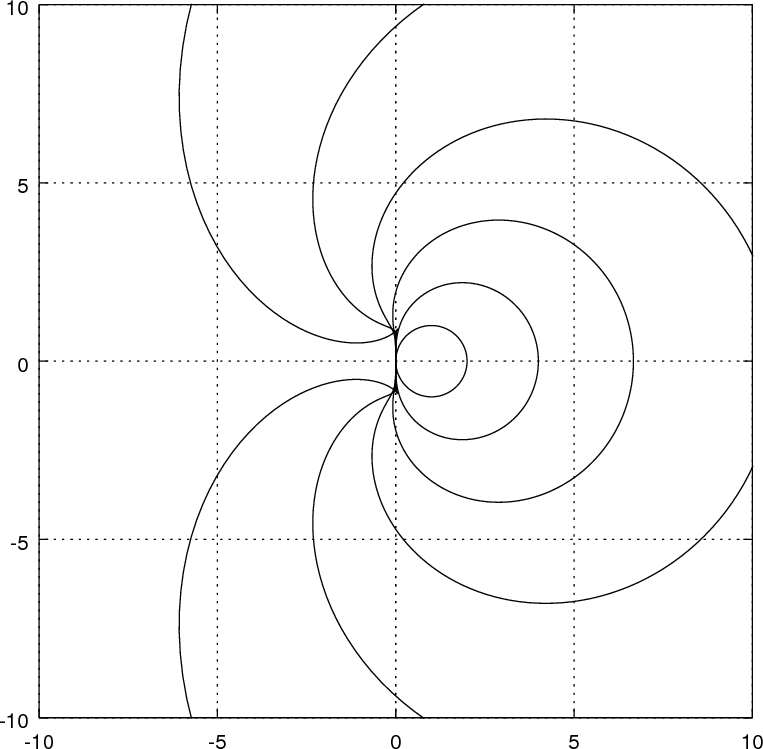
\includegraphics[width=.45\textwidth]{fig/stability-bdf.png}
  \hfill
  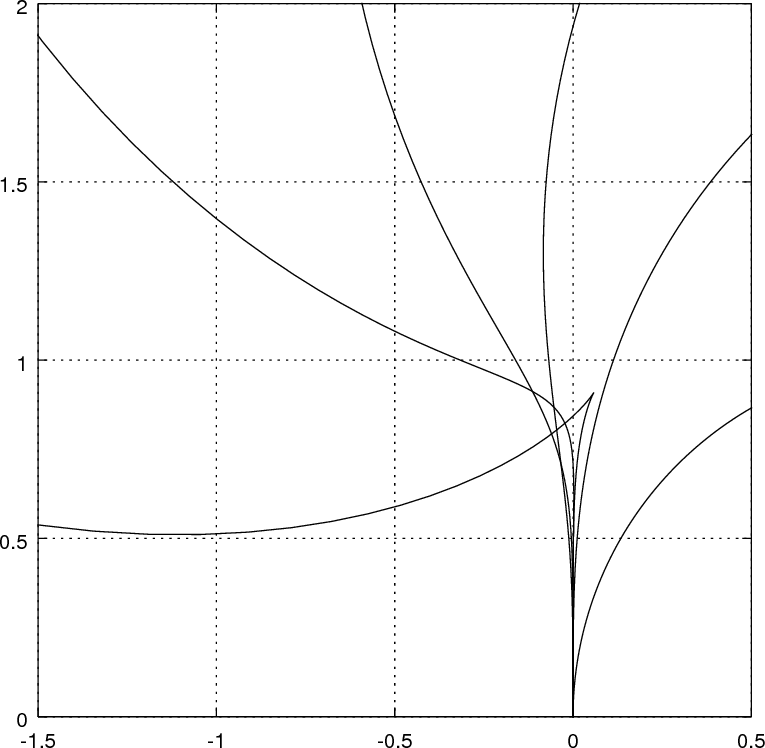
\includegraphics[width=.45\textwidth]{fig/stability-bdf-zoom.png}
  \caption{Boundaries of stability regions of BDF1 to BDF6. Unstable
    region right of the origin. Zoom on the right}
  \label{fig:bdf-stability}
\end{figure}
\begin{table}[tp]
  \centering
  \begin{tabular}{c|cccccc}
    $k$ & 1 & 2 & 3 & 4 & 5 & 6 \\\hline
    $\alpha$ & 90$^\circ$ & 90$^\circ$& 86.03$^\circ$
                    & 73.35$^\circ$& 51.84$^\circ$
                            & 17.84$^\circ$ \\
    $D$ & 0 & 0 & 0.083& 0.667& 2.327& 6.075
  \end{tabular}
  \caption{Values for A($\alpha$)- and stiff stability for BDF methods
    of order $k$.}
  \label{tab:bdf-stability}
\end{table}

%%%%%%%%%%%%%%%%%%%%%%%%%%%%%%%%%%%%%%%%%%%%%%%%%%%%%%%%%%%%%%%%%%%%%%
\section{Predictor-corrector schemes}

\begin{Definition*}{predictor-corrector}{Predictor-corrector methods}
  Assume a pair of time stepping schemes, one explicit, one implicit,
  \begin{align*}
    \hat y_{k} &= \hat \verfahren_p(y_{k-1}) \\
    y_k &= \verfahren_c(y_{k-1},y_{k}),
  \end{align*}
  we can use $\hat y_k$ as initial value for the Newton iteration for
  $y_k$. In an extreme case, we let
  \begin{gather*}
    y_k = \verfahren_c(y_{k-1},\hat y_{k}),
  \end{gather*}
  without any further iteration.
\end{Definition*}

\begin{remark}
  Predictor-corrector methods were developed strongly around
  Adams-Moulton and Adams-Bashforth methods, since the implicit ones
  have much smaller error constants. Given that these methods offer no
  considerable advantages compared to Runge-Kutta methods, but
  stability properties and implementation are weak points, We omit
  their discussion.

  A simple predictor for BDF methods can be obtained, since they are
  based on an interpolating polynomial. Thus, we simply extrapolate
  this polynomial to the next point in time.
\end{remark}

\begin{example}
  While the predictor-corrector idea sounds reasonable, we have to be
  careful with stiff problems, the original reason for using implicit
  methods. Take again our favorite IVP
  \begin{gather*}
    u' = \lambda u,
    \qquad u(0) = 1.
  \end{gather*}
  We apply the BDF(1) scheme, namely the implicit Euler method, with
  step size 1. According to its stability
  function~\eqref{eq:impl:stabil:impleuler}, we obtain
  \begin{gather*}
    y_1 = \frac1{1-\lambda}.
  \end{gather*}
  Accordingly, the interpolating polynomial is
  \begin{gather*}
    y(t) = (1-t) + \frac1{1-\lambda} t = 1 + \frac{\lambda}{1-\lambda}t.
  \end{gather*}
  For the mildly stiff problem $\lambda = -3$, we obtain
  \begin{gather*}
    y_1 = 0.25, \qquad y_2 = 0.0625,
    \qquad \hat y_2 = y(2) = -0.5.
  \end{gather*}
  Thus, the extrapolated value is already a much worse initial value
  for a Newton iteration than using the value from the previous time
  step.
  
  While this example was particularly chosen to exhibit such failure,
  it does show that extrapolation of stiff problems has its
  pitfalls. Here, we end up with a time step restriction which is
  comparable to the stability condition of the explicit method.
\end{example}


%%% Local Variables: 
%%% mode: latex
%%% TeX-master: "notes"
%%% End: 
